This section explains the main identified use cases, presenting each one through a table and a sequence diagram.
The tables outline entry conditions, event flow, exit conditions and exceptions, while the sequence diagrams illustrate the messages exchanged between entities and the functions called.

\newcounter{uc}
\setcounter{uc}{1}

\clearpage
\subsubsection{User Use Cases}
The following use case diagram illustrates the key actions a generic user can perform.

\begin{figure}[h]
    \centering
    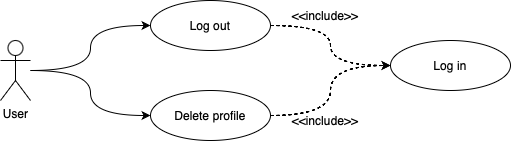
\includegraphics[width=10cm]{images/use-case-diagrams/user.png}
    \caption{User use cases diagram}
\end{figure}

\clearpage
\begin{usecase}
    {UC\theuc. User Logs In}
    {User}
    {The user is signed up on S\&C.}
    {\begin{enumerate}[leftmargin=*]
        \item The user navigates to the landing page.
        \item S\&C displays the landing page.
        \item The user clicks the "Log In" button.
        \item S\&C displays the login page.
        \item The user enters his email address and password.
        \item The user clicks the "Log In" button.
        \item S\&C validates the credentials.
        \item S\&C displays the home page.
    \end{enumerate}}
    {The user is logged in and S\&C displays the home page.}
    {\begin{itemize}[leftmargin=*, label=\tiny\textbullet]
        \item The email address is invalid.
        \item The password in wrong.
        \end{itemize}
        In all cases, S\&C displays a descriptive error message.}
    {Use case \theuc}
\end{usecase}

\begin{figure}
    \centering
    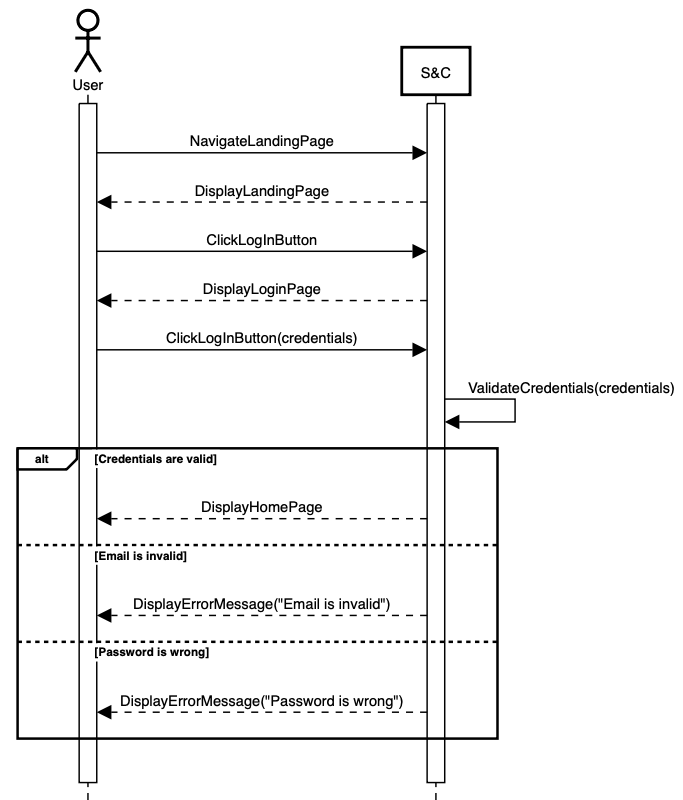
\includegraphics[width=12cm]{images/sequence-diagrams/user-logs-in.png}
    \caption{UC\theuc\ sequence diagram}
\end{figure}

\stepcounter{uc}

\clearpage
\begin{longtable}{|l|p{10.5cm}|}
    \hline \rowcolor{polimiblue!40}
    \multicolumn{2}{|c|}{\textbf{UC\theuc. User Logs Out}} \\ \hline
    \textbf{Actors} & User \\ \hline
    \textbf{Entry Condition} & The user is logged in and S\&C displays the home page. \\ \hline
    \textbf{Event Flow} &
        \begin{minipage}[t]{\linewidth}
            \vspace{10pt}
            \vspace{-\baselineskip}
            \begin{enumerate}[leftmargin=*]
                \item The user clicks the "My Profile" button.
                \item S\&C displays the profile page.
                \item The user clicks the "Log Out" button.
                \item S\&C displays the landing page.
            \end{enumerate}
            \vspace{10pt}
        \end{minipage} \\ \hline
    \textbf{Exit Condition} & The user is logged out and S\&C displays the landing page. \\ \hline
    \textbf{Exceptions} &
        \begin{minipage}[t]{\linewidth}
            \vspace{10pt}
            \vspace{-\baselineskip}
            None.
            \vspace{10pt}
        \end{minipage} \\ \hline
\caption{Use case \theuc}
\end{longtable}

\begin{figure}[h]
    \centering
    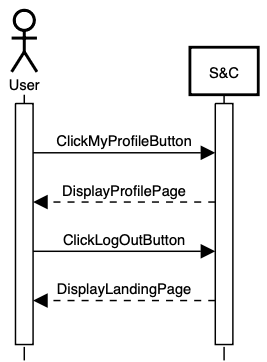
\includegraphics[width=5cm]{images/sequence-diagrams/user-logs-out.png}
    \caption{UC\theuc\ sequence diagram}
\end{figure}

\stepcounter{uc}

\clearpage
\begin{longtable}{|l|p{10.5cm}|}
    \hline \rowcolor{polimiblue!40}
    \multicolumn{2}{|c|}{\textbf{UC\theuc. User Deletes Profile}} \\ \hline
    \textbf{Actors} & User, EP \\ \hline
    \textbf{Entry Condition} & The user is logged in and S\&C displays the home page. \\ \hline
    \textbf{Event Flow} &
        \begin{minipage}[t]{\linewidth}
            \vspace{10pt}
            \vspace{-\baselineskip}
            \begin{enumerate}[leftmargin=*]
                \item The user clicks the "My Profile" button.
                \item S\&C displays the profile page.
                \item The user clicks the "Delete Profile" button.
                \item S\&C sends a confirmation email to the user via the EP.
                \item The user clicks the confirmation link in the email.
                \item S\&C displays the landing page.
            \end{enumerate}
            \vspace{10pt}
        \end{minipage} \\ \hline
    \textbf{Exit Condition} & The profile is deleted and S\&C displays the landing page. \\ \hline
    \textbf{Exceptions} &
        \begin{minipage}[t]{\linewidth}
            \vspace{10pt}
            \vspace{-\baselineskip}
            None.
            \vspace{10pt}
        \end{minipage} \\ \hline
\caption{Use case \theuc}
\end{longtable}

\begin{figure}[h]
    \centering
    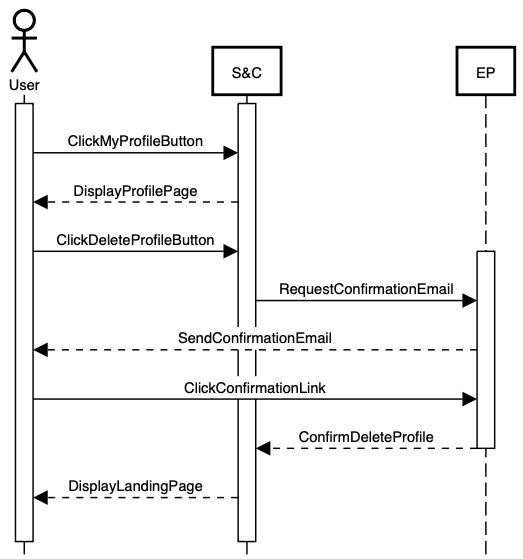
\includegraphics[width=9cm]{images/sequence-diagrams/user-deletes-profile.png}
    \caption{UC\theuc\ sequence diagram}
\end{figure}

\stepcounter{uc}

\clearpage
\subsubsection{Student Use Cases}
The following use case diagram outlines the main interactions a student can have.

\begin{figure}[h]
   \centering    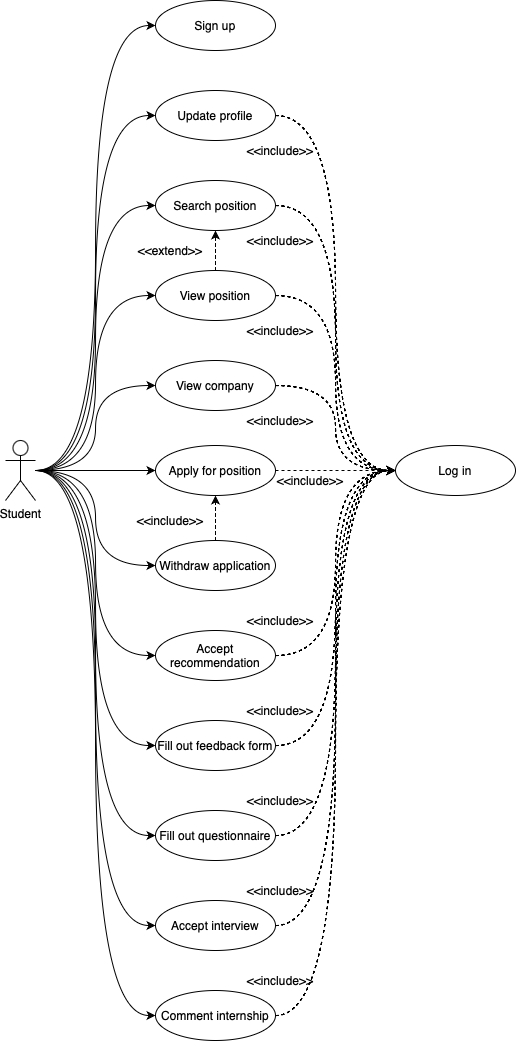
\includegraphics[width=10cm]{images/use-case-diagrams/student.png}
    \caption{Student use cases diagram}
\end{figure}

\clearpage
\begin{longtable}{|l|p{10.5cm}|}
    \hline \rowcolor{polimiblue!40}
    \multicolumn{2}{|c|}{\textbf{UC\theuc. Student Signs Up}} \\ \hline
    \textbf{Actors} & US, EP \\ \hline
    \textbf{Entry Condition} & The US is not signed up on S\&C. \\ \hline
    \textbf{Event Flow} &
        \begin{minipage}[t]{\linewidth}
            \vspace{10pt}
            \vspace{-\baselineskip}
            \begin{enumerate}[leftmargin=*]
                \item The US navigates to the landing page.
                \item S\&C displays the landing page.
                \item The US clicks the "Sign Up as a Student" button.
                \item S\&C displays the signup page.
                \item The US enters his name, surname, institutional email address, password and confirms the password.
                \item The US can upload a CV and enter preferences.
                \item The US can tick the "Keep Me Updated" field.
                \item The US clicks the "Sign Up" button.
                \item S\&C validates the fields.
                \item S\&C sends a confirmation email to the US via the EP.
                \item The US clicks the confirmation link in the email.
                \item S\&C displays the login page.
            \end{enumerate}
            \vspace{10pt}
        \end{minipage} \\ \hline
    \textbf{Exit Condition} & The US is signed up and S\&C displays the login page. \\ \hline
    \textbf{Exceptions} &
        \begin{minipage}[t]{\linewidth}
            \vspace{10pt}
            \vspace{-\baselineskip}
            \begin{itemize}[leftmargin=*, label=\tiny\textbullet]
                \item The email is not a valid institutional email address.
                \item The email is already linked to another profile.
                \item The password is shorter than 8 characters.
                \item The passwords do not match.
                \item Another field is invalid.
            \end{itemize}
            In all cases, S\&C displays a descriptive error message.
            \vspace{10pt}
        \end{minipage} \\ \hline
\caption{Use case \theuc}
\end{longtable}

\begin{figure}
    \centering
    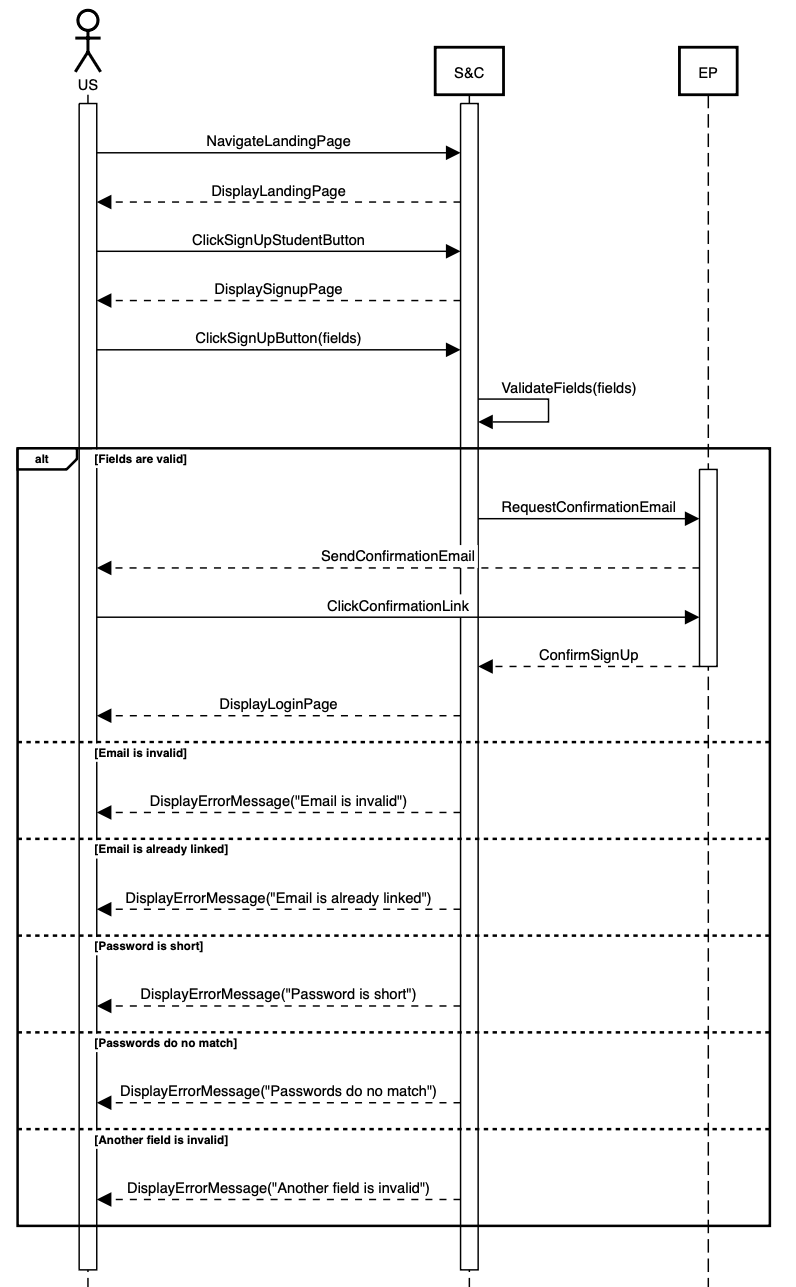
\includegraphics[width=13cm]{images/sequence-diagrams/student-signs-up.png}
    \caption{UC\theuc\ sequence diagram}
\end{figure}

\stepcounter{uc}

\clearpage
\begin{longtable}{|l|p{10.5cm}|}
    \hline \rowcolor{polimiblue!40}
    \multicolumn{2}{|c|}{\textbf{UC\theuc. Student Updates Profile}} \\ \hline
    \textbf{Actors} & US \\ \hline
    \textbf{Entry Condition} & The US is logged in and S\&C displays the home page. \\ \hline
    \textbf{Event Flow} &
        \begin{minipage}[t]{\linewidth}
            \vspace{10pt}
            \vspace{-\baselineskip}
            \begin{enumerate}[leftmargin=*]
                \item The US clicks the "My Profile" button.
                \item S\&C displays the profile page.
                \item The US clicks the "Update Profile" button.
                \item S\&C displays the profile editor.
                \item The US updates the desired fields.
                \item The US clicks the "Save Profile" button.
                \item S\&C validates the fields.
                \item S\&C displays the profile page.
            \end{enumerate}
            \vspace{10pt}
        \end{minipage} \\ \hline
    \textbf{Exit Condition} & The profile is updated and S\&C displays the profile page. \\ \hline
    \textbf{Exceptions} &
        \begin{minipage}[t]{\linewidth}
            \vspace{10pt}
            \vspace{-\baselineskip}
            \begin{itemize}[leftmargin=*, label=\tiny\textbullet]
                \item The email is not a valid institutional email address.
                \item The email is already linked to another profile.
                \item The password is shorter than 8 characters.
                \item The passwords do not match.
                \item Another field is invalid.
            \end{itemize}
            In all cases, S\&C displays a descriptive error message.
            \vspace{10pt}
        \end{minipage} \\ \hline
\caption{Use case \theuc}
\end{longtable}

\begin{figure}
    \centering
    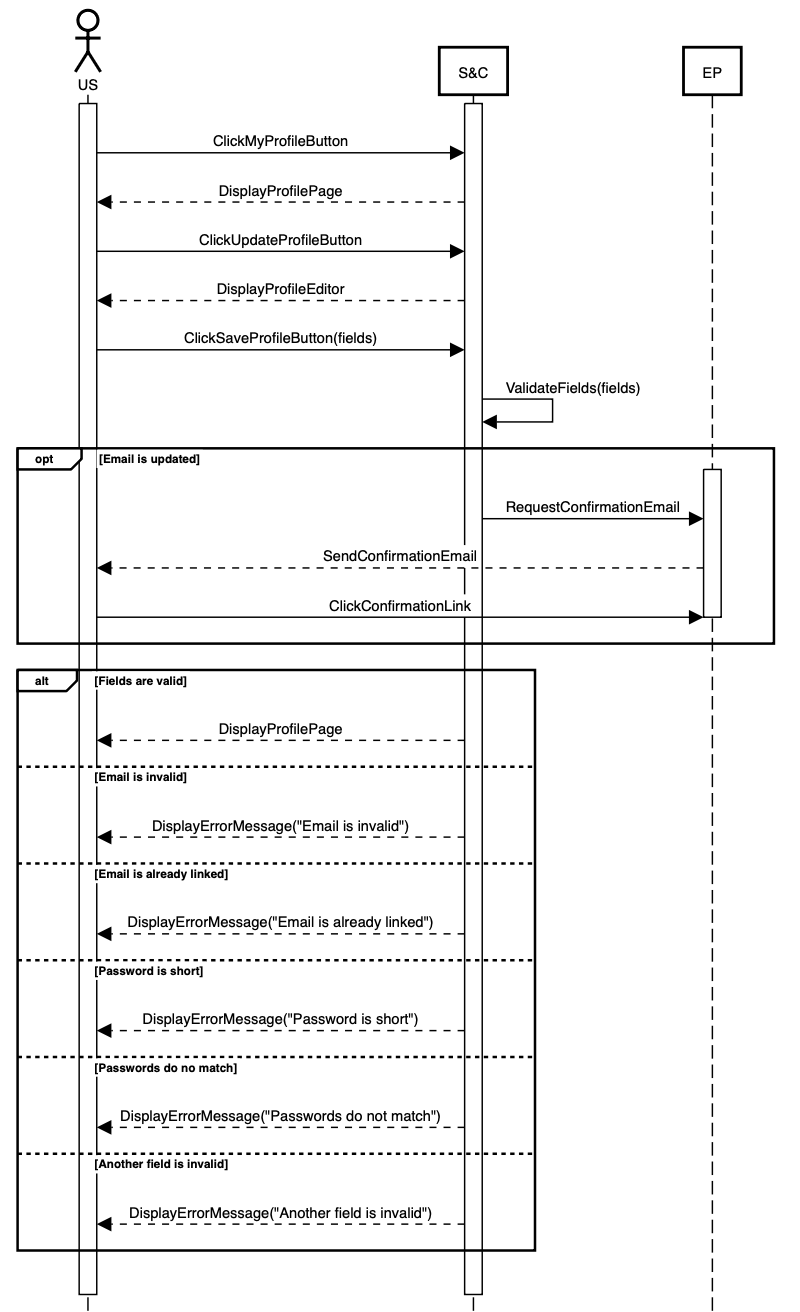
\includegraphics[width=14cm]{images/sequence-diagrams/student-updates-profile.png}
    \caption{UC\theuc\ sequence diagram}
\end{figure}

\stepcounter{uc}

\clearpage
\begin{longtable}{|l|p{10.5cm}|}
    \hline \rowcolor{polimiblue!40}
    \multicolumn{2}{|c|}{\textbf{UC\theuc. Student Searches Position}} \\ \hline
    \textbf{Actors} & US \\ \hline
    \textbf{Entry Condition} & The US is logged in and S\&C displays the home page. \\ \hline
    \textbf{Event Flow} &
        \begin{minipage}[t]{\linewidth}
            \vspace{10pt}
            \vspace{-\baselineskip}
            \begin{enumerate}[leftmargin=*]
                \item The US enters a keyword in the search bar.
                \item The US clicks the "Search" button.
                \item S\&C computes the results.
                \item S\&C displays the results page.
            \end{enumerate}
            \vspace{10pt}
        \end{minipage} \\ \hline
    \textbf{Exit Condition} & S\&C displays the results page. \\ \hline
    \textbf{Exceptions} &
        \begin{minipage}[t]{\linewidth}
            \vspace{10pt}
            \vspace{-\baselineskip}
            \begin{itemize}[leftmargin=*, label=\tiny\textbullet]
                \item No results are computed.
            \end{itemize}
            In this case, S\&C displays a descriptive error message.
            \vspace{10pt}
        \end{minipage} \\ \hline
\caption{Use case \theuc}
\end{longtable}

\begin{figure}[h]
    \centering
    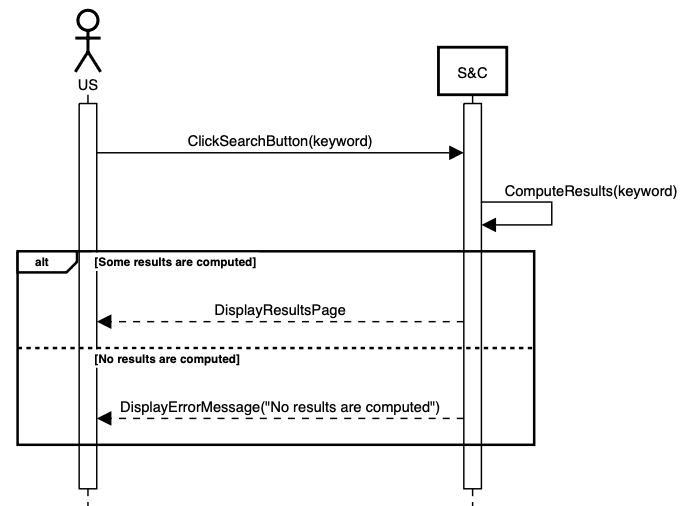
\includegraphics[width=13cm]{images/sequence-diagrams/student-searches-position.png}
    \caption{UC\theuc\ sequence diagram}
\end{figure}

\stepcounter{uc}

\clearpage
\begin{longtable}{|l|p{10.5cm}|}
    \hline \rowcolor{polimiblue!40}
    \multicolumn{2}{|c|}{\textbf{UC\theuc. Student Views Position}} \\ \hline
    \textbf{Actors} & US \\ \hline
    \textbf{Entry Condition} & The US is logged in and S\&C displays the PO name. \\ \hline
    \textbf{Event Flow} &
        \begin{minipage}[t]{\linewidth}
            \vspace{10pt}
            \vspace{-\baselineskip}
            \begin{enumerate}[leftmargin=*]
                \item The US clicks the PO name.
                \item S\&C displays the PO page.
            \end{enumerate}
            \vspace{10pt}
        \end{minipage} \\ \hline
    \textbf{Exit Condition} & S\&C displays the PO page. \\ \hline
    \textbf{Exceptions} &
        \begin{minipage}[t]{\linewidth}
            \vspace{10pt}
            \vspace{-\baselineskip}
            \begin{itemize}[leftmargin=*, label=\tiny\textbullet]
                \item The PO has been removed.
                \item The CO has been deleted.
            \end{itemize}
            In all cases, S\&C displays a descriptive error message.
            \vspace{10pt}
        \end{minipage} \\ \hline
\caption{Use case \theuc}
\end{longtable}

\begin{figure}[h]
    \centering
    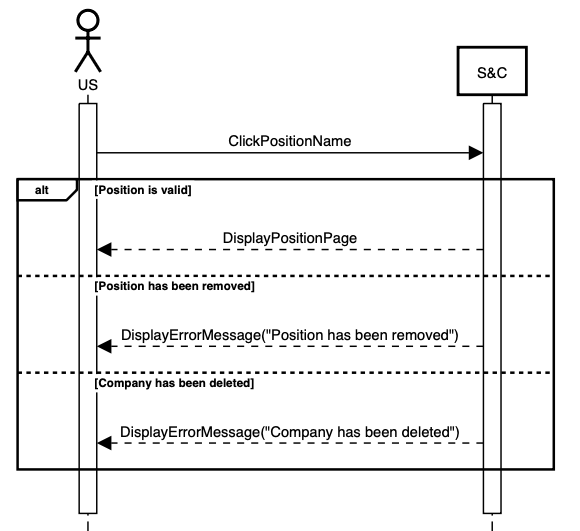
\includegraphics[width=11cm]{images/sequence-diagrams/student-views-position.png}
    \caption{UC\theuc\ sequence diagram}
\end{figure}

\stepcounter{uc}

\clearpage
\begin{longtable}{|l|p{10.5cm}|}
    \hline \rowcolor{polimiblue!40}
    \multicolumn{2}{|c|}{\textbf{UC\theuc. Student Views Company}} \\ \hline
    \textbf{Actors} & US \\ \hline
    \textbf{Entry Condition} & The US is logged in and S\&C displays the CO name. \\ \hline
    \textbf{Event Flow} &
        \begin{minipage}[t]{\linewidth}
            \vspace{10pt}
            \vspace{-\baselineskip}
            \begin{enumerate}[leftmargin=*]
                \item The US clicks the CO name.
                \item S\&C displays the CO page.
            \end{enumerate}
            \vspace{10pt}
        \end{minipage} \\ \hline
    \textbf{Exit Condition} & S\&C displays the CO page. \\ \hline
    \textbf{Exceptions} &
        \begin{minipage}[t]{\linewidth}
            \vspace{10pt}
            \vspace{-\baselineskip}
            \begin{itemize}[leftmargin=*, label=\tiny\textbullet]
                \item The CO has been deleted.
            \end{itemize}
            In this case, S\&C displays a descriptive error message.
            \vspace{10pt}
        \end{minipage} \\ \hline
\caption{Use case \theuc}
\end{longtable}

\begin{figure}[h]
    \centering
    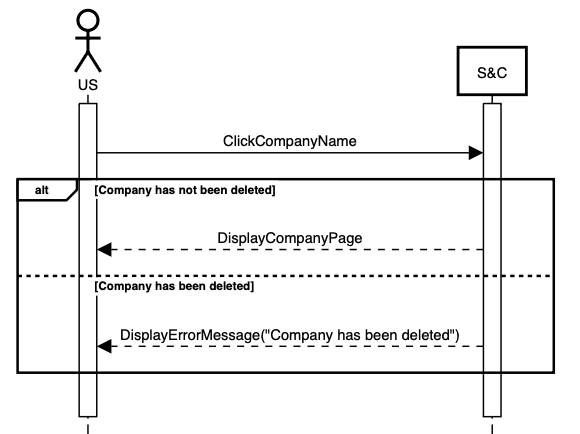
\includegraphics[width=11cm]{images/sequence-diagrams/student-views-company.png}
    \caption{UC\theuc\ sequence diagram}
\end{figure}

\stepcounter{uc}

\clearpage
\begin{longtable}{|l|p{10.5cm}|}
    \hline \rowcolor{polimiblue!40}
    \multicolumn{2}{|c|}{\textbf{UC\theuc. Student Applies for Position}} \\ \hline
    \textbf{Actors} & US, CO, EP \\ \hline
    \textbf{Entry Condition} & The US is logged in and S\&C displays the PO page. \\ \hline
    \textbf{Event Flow} &
        \begin{minipage}[t]{\linewidth}
            \vspace{10pt}
            \vspace{-\baselineskip}
            \begin{enumerate}[leftmargin=*]
                \item The US clicks the "Apply" button.
                \item S\&C displays the application page.
                \item S\&C sends a confirmation email to the US via the EP.
                \item S\&C sends a notification email to the CO via the EP.
            \end{enumerate}
            \vspace{10pt}
        \end{minipage} \\ \hline
    \textbf{Exit Condition} & The US has applied for the PO, the CO has been notified and S\&C displays the application page. \\ \hline
    \textbf{Exceptions} &
        \begin{minipage}[t]{\linewidth}
            \vspace{10pt}
            \vspace{-\baselineskip}
            \begin{itemize}[leftmargin=*, label=\tiny\textbullet]
                \item The US has already applied.
                \item The PO has been removed.
                \item The CO has been deleted.
            \end{itemize}
            In all cases, S\&C displays a descriptive error message.
            \vspace{10pt}
        \end{minipage} \\ \hline
\caption{Use case \theuc}
\end{longtable}

\begin{figure}[h]
    \centering
    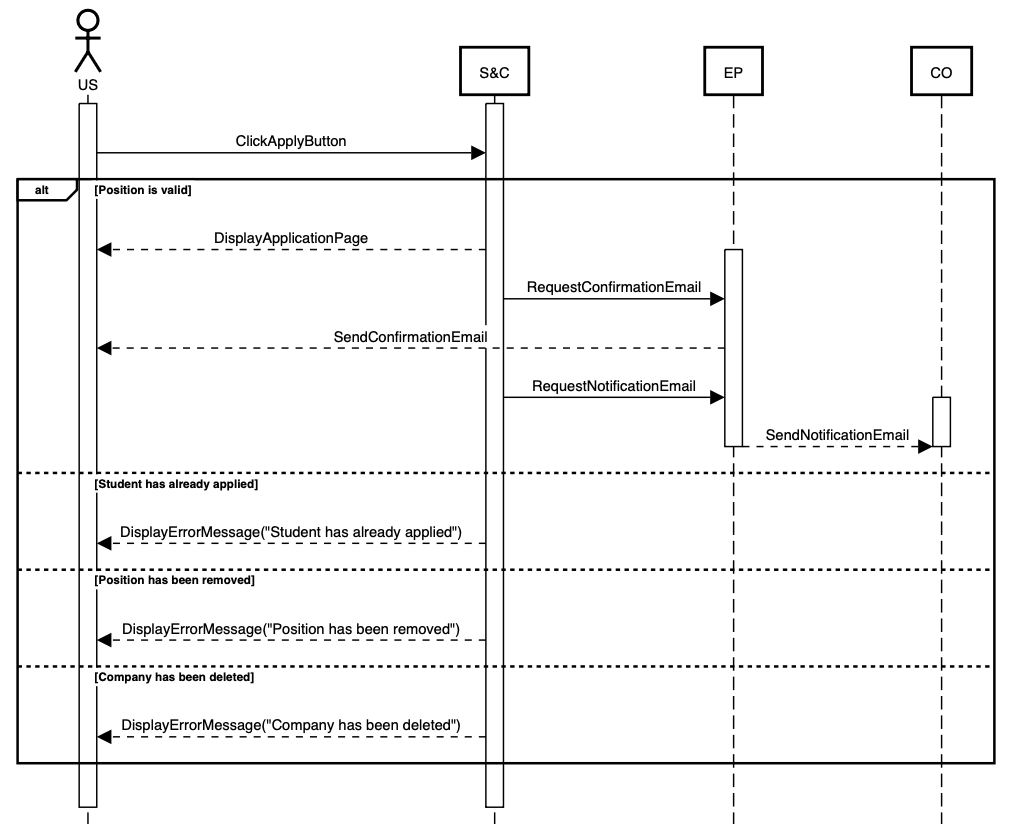
\includegraphics[width=16cm]{images/sequence-diagrams/student-applies-for-position.png}
    \caption{UC\theuc\ sequence diagram}
\end{figure}

\stepcounter{uc}

\clearpage
\begin{longtable}{|l|p{10.5cm}|}
    \hline \rowcolor{polimiblue!40}
    \multicolumn{2}{|c|}{\textbf{UC\theuc. Student Withdraws Application}} \\ \hline
    \textbf{Actors} & US \\ \hline
    \textbf{Entry Condition} & The US is logged in, has applied for the PO and S\&C displays the home page. \\ \hline
    \textbf{Event Flow} &
        \begin{minipage}[t]{\linewidth}
            \vspace{10pt}
            \vspace{-\baselineskip}
            \begin{enumerate}[leftmargin=*]
                \item The US clicks the "My Applications" button.
                \item S\&C displays the applications page.
                \item The US clicks the application name.
                \item S\&C displays the application page.
                \item The US clicks the "Withdraw" button.
                \item S\&C displays the "My Applications" page.
            \end{enumerate}
            \vspace{10pt}
        \end{minipage} \\ \hline
    \textbf{Exit Condition} & The application is withdrawn and S\&C displays the "My Applications" page. \\ \hline
    \textbf{Exceptions} &
        \begin{minipage}[t]{\linewidth}
            \vspace{10pt}
            \vspace{-\baselineskip}
            None.
            \vspace{10pt}
        \end{minipage} \\ \hline
\caption{Use case \theuc}
\end{longtable}

\begin{figure}[h]
    \centering
    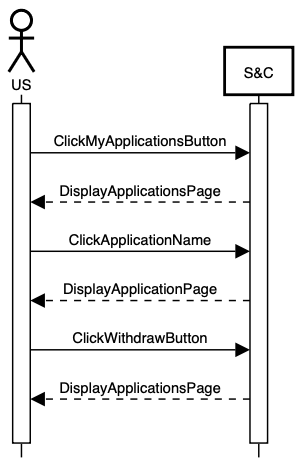
\includegraphics[width=6cm]{images/sequence-diagrams/student-withdraws-application.png}
    \caption{UC\theuc\ sequence diagram}
\end{figure}

\stepcounter{uc}

\clearpage
\begin{longtable}{|l|p{10.5cm}|}
    \hline \rowcolor{polimiblue!40}
    \multicolumn{2}{|c|}{\textbf{UC\theuc. Students Accepts Recommendation}} \\ \hline
    \textbf{Actors} & US, CO, EP \\ \hline
    \textbf{Entry Condition} & The US is logged in, has uploaded a CV, entered preferences and ticked the "Keep Me Updated" field. \\ \hline
    \textbf{Event Flow} &
        \begin{minipage}[t]{\linewidth}
            \vspace{10pt}
            \vspace{-\baselineskip}
            \begin{enumerate}[leftmargin=*]
                \item S\&C sends a notification email to the US via the EP.
                \item The US clicks the "View Position" link on the email.
                \item S\&C displays the PO page.
                \item The US clicks the "Accept" button.
                \item S\&C displays the application page.
                \item S\&C checks if a match is identified.
                \item S\&C sends a notification email to the US via the EP.
                \item S\&C sends a notification email to the CO via the EP.
            \end{enumerate}
            \vspace{10pt}
        \end{minipage} \\ \hline
    \textbf{Exit Condition} & The recommendation is accepted and S\&C displays the application page. \\ \hline
    \textbf{Exceptions} &
        \begin{minipage}[t]{\linewidth}
            \vspace{10pt}
            \vspace{-\baselineskip}
            \begin{itemize}[leftmargin=*, label=\tiny\textbullet]
                \item The recommendation has already been resolved.
                \item The PO has been removed.
                \item The CO has been deleted.
            \end{itemize}
            In all cases, S\&C displays the home page and a descriptive error message.
            \vspace{10pt}
        \end{minipage} \\ \hline
\caption{Use case \theuc}
\end{longtable}

\begin{figure}
    \centering
    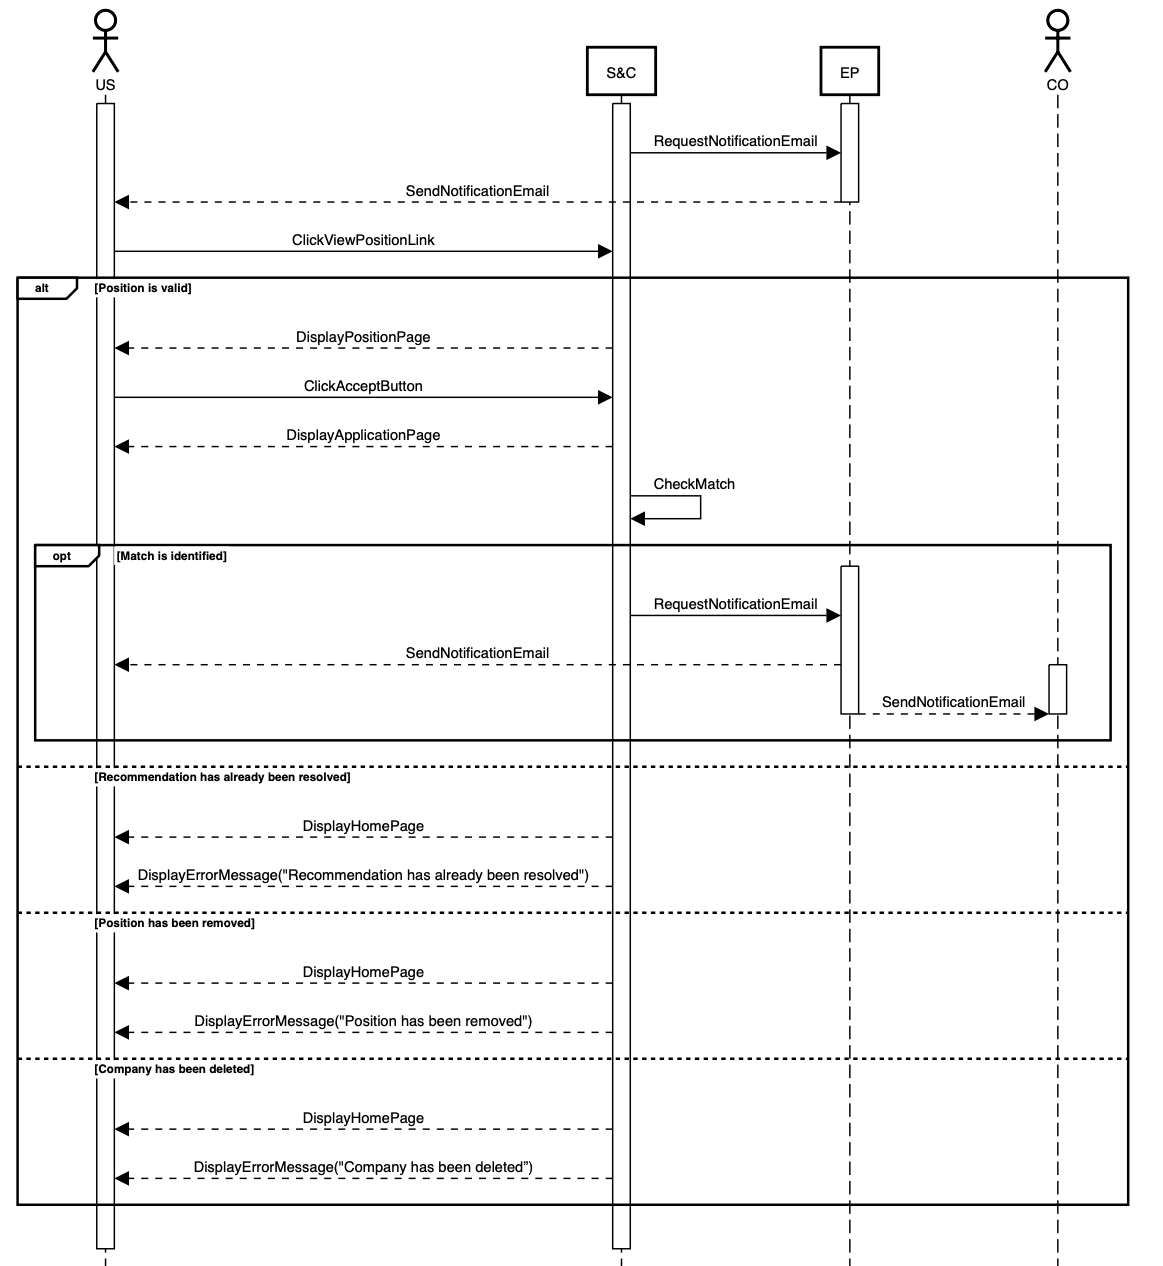
\includegraphics[width=16cm]{images/sequence-diagrams/student-accepts-recommendation.png}
    \caption{UC\theuc\ sequence diagram}
\end{figure}

\stepcounter{uc}

\clearpage
\begin{longtable}{|l|p{10.5cm}|}
    \hline \rowcolor{polimiblue!40}
    \multicolumn{2}{|c|}{\textbf{UC\theuc. Student Fills Out Feedback Form}} \\ \hline
    \textbf{Actors} & US \\ \hline
    \textbf{Entry Condition} & The US is logged in and S\&C displays the home page. \\ \hline
    \textbf{Event Flow} &
        \begin{minipage}[t]{\linewidth}
            \vspace{10pt}
            \vspace{-\baselineskip}
            \begin{enumerate}[leftmargin=*]
                \item The US clicks the "Give Feedback" button.
                \item S\&C displays the feedback form.
                \item The US enters the fields.
                \item The US clicks the "Submit" button.
                \item S\&C validates the fields.
                \item S\&C displays the home page.
            \end{enumerate}
            \vspace{10pt}
        \end{minipage} \\ \hline
    \textbf{Exit Condition} & The feedback form is submitted and S\&C displays the home page. \\ \hline
    \textbf{Exceptions} &
        \begin{minipage}[t]{\linewidth}
            \vspace{10pt}
            \vspace{-\baselineskip}
            \begin{itemize}[leftmargin=*, label=\tiny\textbullet]
                \item A field is invalid.
            \end{itemize}
            In this case, S\&C displays a descriptive error message.
            \vspace{10pt}
        \end{minipage} \\ \hline
\caption{Use case \theuc}
\end{longtable}

\begin{figure}[h]
    \centering
    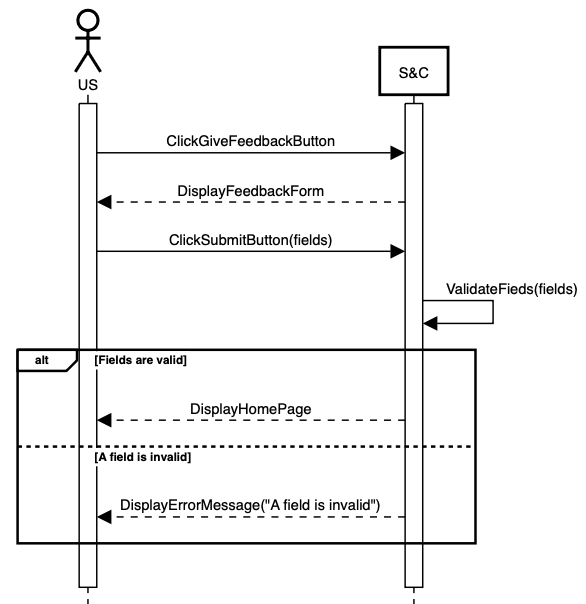
\includegraphics[width=11cm]{images/sequence-diagrams/student-fills-out-feedback-form.png}
    \caption{UC\theuc\ sequence diagram}
\end{figure}

\stepcounter{uc}

\clearpage
\begin{longtable}{|l|p{10.5cm}|}
    \hline \rowcolor{polimiblue!40}
    \multicolumn{2}{|c|}{\textbf{UC\theuc. Student Fills Out Questionnaire}} \\ \hline
    \textbf{Actors} & US, CO, EP \\ \hline
    \textbf{Entry Conditions} & The US is logged in, has received a notification on an added questionnaire and S\&C displays the home page. \\ \hline
    \textbf{Event Flow} &
        \begin{minipage}[t]{\linewidth}
            \vspace{10pt}
            \vspace{-\baselineskip}
            \begin{enumerate}[leftmargin=*]
                \item The US clicks the "My Applications" button.
                \item S\&C displays the applications page.
                \item The US clicks the application name.
                \item S\&C displays the application page.
                \item The US clicks the "View Questionnaire" button.
                \item S\&C displays the questionnaire.
                \item The US enters the fields.
                \item The US clicks the "Submit" button.
                \item S\&C validates the fields.
                \item S\&C displays the application page.
                \item S\&C sends a notification email to the CO via the EP.
            \end{enumerate}
            \vspace{10pt}
        \end{minipage} \\ \hline
    \textbf{Exit Condition} & The questionnaire is submitted and S\&C displays the application page. \\ \hline
    \textbf{Exceptions} &
        \begin{minipage}[t]{\linewidth}
            \vspace{10pt}
            \vspace{-\baselineskip}
            \begin{itemize}[leftmargin=*, label=\tiny\textbullet]
                \item A field is invalid.
            \end{itemize}
            In this case, S\&C displays a descriptive error message.
            \vspace{10pt}
        \end{minipage} \\ \hline
\caption{Use case \theuc}
\end{longtable}

\begin{figure}
    \centering
    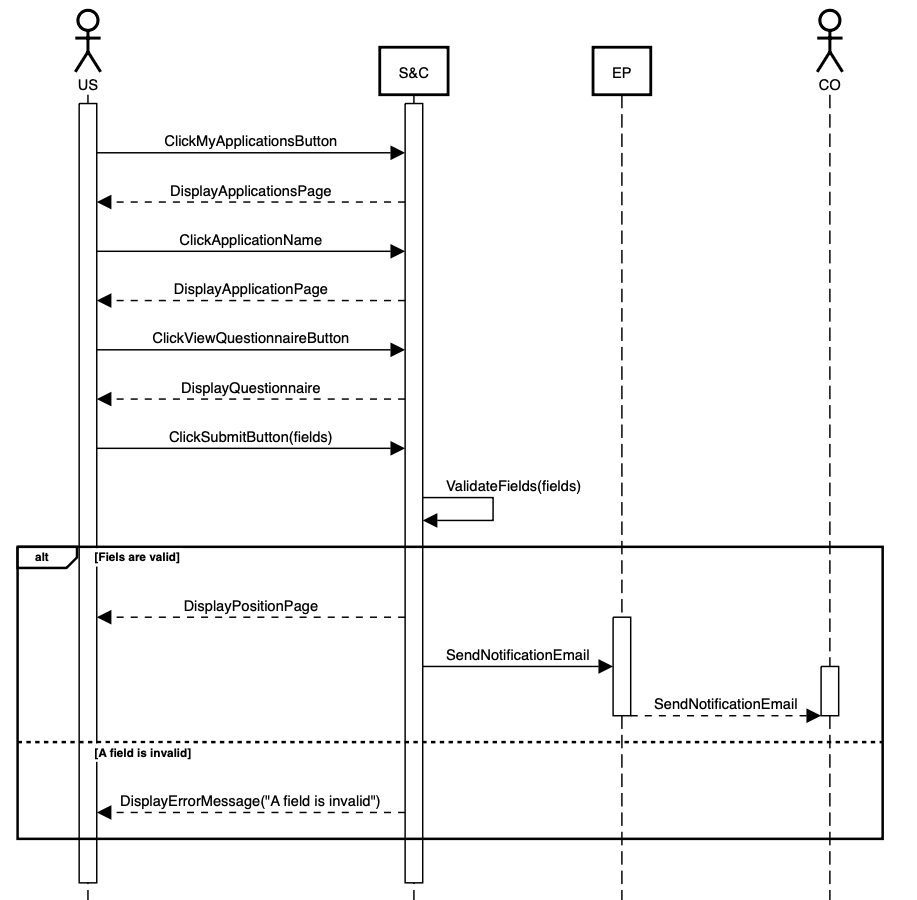
\includegraphics[width=16cm]{images/sequence-diagrams/student-fills-out-questionnaire.png}
    \caption{UC\theuc\ sequence diagram}
\end{figure}

\stepcounter{uc}

\clearpage
\begin{longtable}{|l|p{10.5cm}|}
    \hline \rowcolor{polimiblue!40}
    \multicolumn{2}{|c|}{\textbf{UC\theuc. Student Accepts Interview}} \\ \hline
    \textbf{Actors} & US, CO, EP \\ \hline
    \textbf{Entry Conditions} & The US is logged in, has received a notification on a scheduled interview and S\&C displays the home page. \\ \hline
    \textbf{Event Flow} &
        \begin{minipage}[t]{\linewidth}
            \vspace{10pt}
            \vspace{-\baselineskip}
            \begin{enumerate}[leftmargin=*]
                \item The US clicks the "My Applications" button.
                \item S\&C displays the applications page.
                \item The US clicks the application name.
                \item S\&C displays the application page.
                \item The US clicks the "View Interview" button.
                \item S\&C displays the interview page.
                \item The US clicks the "Accept" button.
                \item S\&C displays the application page.
                \item S\&C sends a notification email to the CO via the EP.
            \end{enumerate}
            \vspace{10pt}
        \end{minipage} \\ \hline
    \textbf{Exit Condition} & The interview is scheduled and S\&C displays the application page. \\ \hline
    \textbf{Exceptions} &
        \begin{minipage}[t]{\linewidth}
            \vspace{10pt}
            \vspace{-\baselineskip}
            None.
            \vspace{10pt}
        \end{minipage} \\ \hline
\caption{Use case \theuc}
\end{longtable}

\begin{figure}
    \centering
    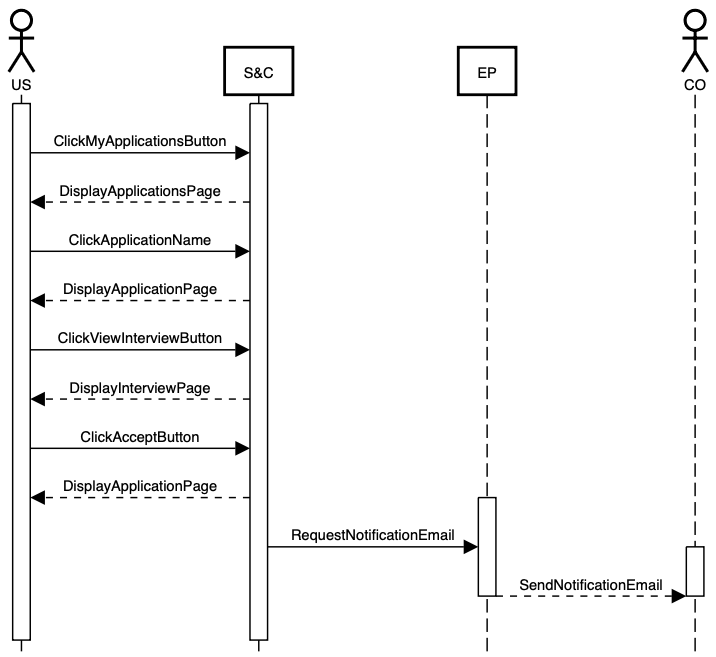
\includegraphics[width=14cm]{images/sequence-diagrams/student-accepts-interview.png}
    \caption{UC\theuc\ sequence diagram}
\end{figure}

\stepcounter{uc}

\clearpage
\begin{longtable}{|l|p{10.5cm}|}
    \hline \rowcolor{polimiblue!40}
    \multicolumn{2}{|c|}{\textbf{UC\theuc. Student Comments Internship}} \\ \hline
    \textbf{Actors} & US, CO, UN, EP \\ \hline
    \textbf{Entry Conditions} & The US is logged in, doing an IN and S\&C displays the home page. \\ \hline
    \textbf{Event Flow} &
        \begin{minipage}[t]{\linewidth}
            \vspace{10pt}
            \vspace{-\baselineskip}
            \begin{enumerate}[leftmargin=*]
                \item The US clicks the "My Internships" button.
                \item S\&C displays the internships page.
                \item The US clicks the IN name.
                \item S\&C displays the IN page.
                \item The US clicks the "Write a Comment" button.
                \item S\&C displays the comment form.
                \item The US enters the fields.
                \item The US clicks the "Send" button.
                \item S\&C validates the fields.
                \item S\&C displays the IN page.
                \item S\&C sends a notification email to the CO via the EP.
                \item S\&C sends a notification email to the UN via the EP.
            \end{enumerate}
            \vspace{10pt}
        \end{minipage} \\ \hline
    \textbf{Exit Condition} & The comment is sent, the CO and the UN are notified and S\&C displays the IN page. \\ \hline
    \textbf{Exceptions} &
        \begin{minipage}[t]{\linewidth}
            \vspace{10pt}
            \vspace{-\baselineskip}
            \begin{itemize}[leftmargin=*, label=\tiny\textbullet]
                \item A field is invalid.
            \end{itemize}
            In this case, S\&C displays a descriptive error message.
            \vspace{10pt}
        \end{minipage} \\ \hline
\caption{Use case \theuc}
\end{longtable}

\begin{figure}
    \centering
    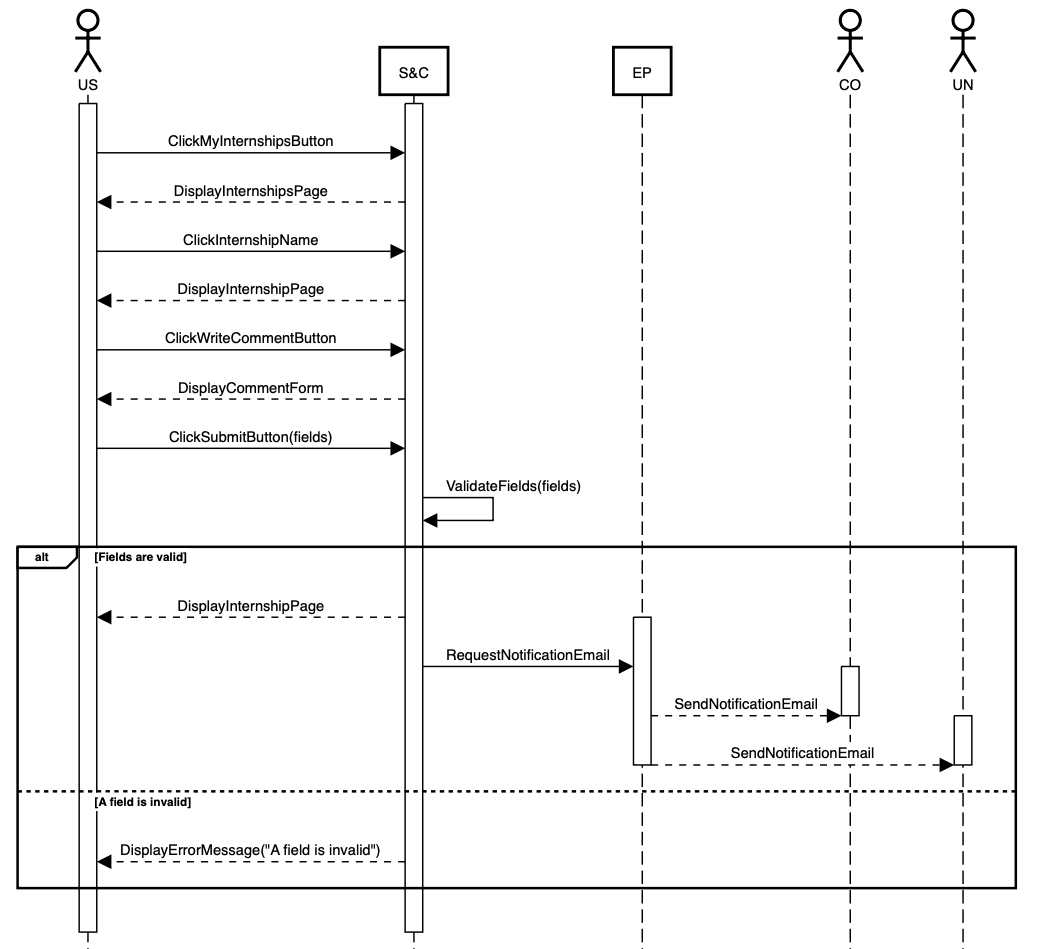
\includegraphics[width=16cm]{images/sequence-diagrams/student-comments-internship.png}
    \caption{UC\theuc\ sequence diagram}
\end{figure}

\stepcounter{uc}

\clearpage
\subsubsection{Company Use Cases}
The use case diagram below demonstrates the primary operations a company can perform.

\begin{figure}[h]
   \centering    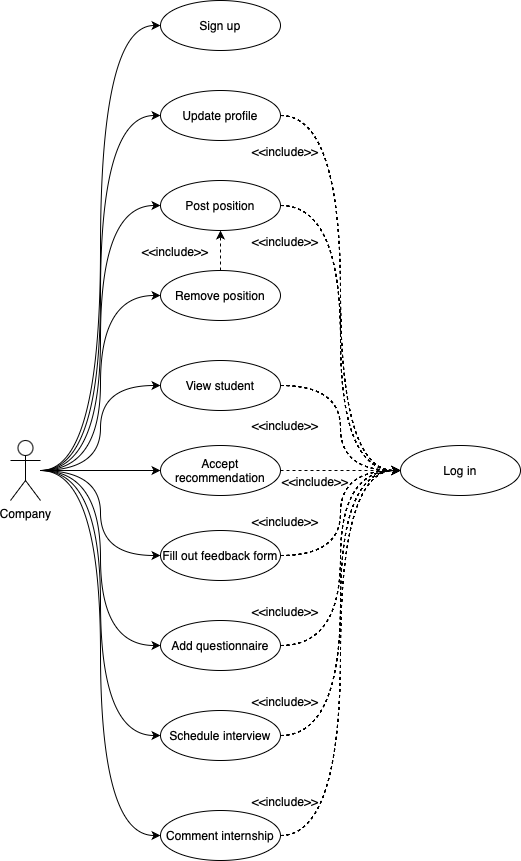
\includegraphics[width=10cm]{images/use-case-diagrams/company.png}
    \caption{Company use cases diagram}
\end{figure}

\clearpage
\begin{longtable}{|l|p{10.5cm}|}
    \hline \rowcolor{polimiblue!40}
    \multicolumn{2}{|c|}{\textbf{UC\theuc. Company Signs Up}} \\ \hline
    \textbf{Actors} & CO, EP \\ \hline
    \textbf{Entry Condition} & The CO is not signed up on S\&C. \\ \hline
    \textbf{Event Flow} &
        \begin{minipage}[t]{\linewidth}
            \vspace{10pt}
            \vspace{-\baselineskip}
            \begin{enumerate}[leftmargin=*]
                \item The CO navigates to the landing page.
                \item S\&C displays the landing page.
                \item The CO clicks the "Sign Up as a Company" button.
                \item S\&C displays the signup page.
                \item The CO enters his name, email address, password and confirms the password.
                \item The CO can tick the "Keep Me Updated" field.
                \item The CO clicks the "Sign Up" button.
                \item S\&C validates the fields.
                \item S\&C sends a confirmation email to the CO via the EP.
                \item The CO clicks the confirmation link in the email.
                \item S\&C displays the login page.
            \end{enumerate}
            \vspace{10pt}
        \end{minipage} \\ \hline
    \textbf{Exit Condition} & The CO is signed up and S\&C displays the login page. \\ \hline
    \textbf{Exceptions} &
        \begin{minipage}[t]{\linewidth}
            \vspace{10pt}
            \vspace{-\baselineskip}
            \begin{itemize}[leftmargin=*, label=\tiny\textbullet]
                \item The email is already linked to another profile.
                \item The password is shorter than 8 characters.
                \item The passwords do not match.
                \item Another field is invalid.
            \end{itemize}
            In all cases, S\&C displays a descriptive error message.
            \vspace{10pt}
        \end{minipage} \\ \hline
\caption{Use case \theuc}
\end{longtable}

\begin{figure}
    \centering
    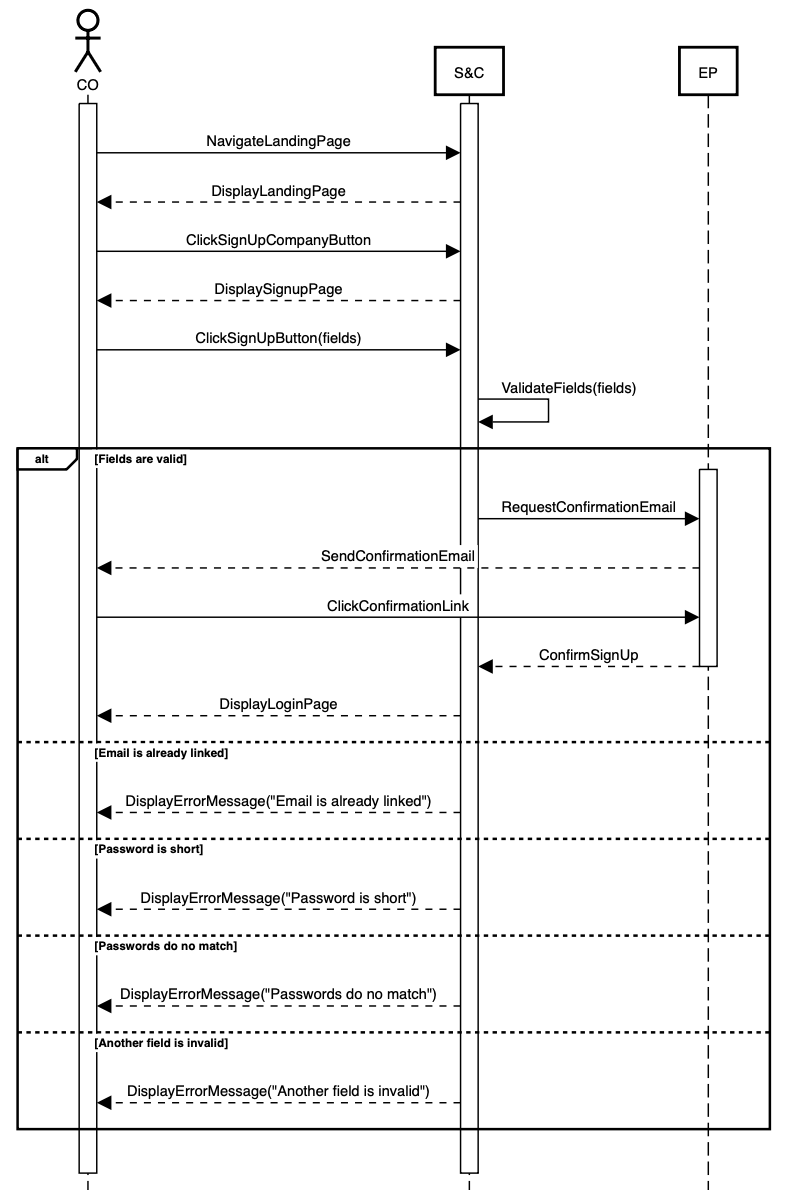
\includegraphics[width=13cm]{images/sequence-diagrams/company-signs-up.png}
    \caption{UC\theuc\ sequence diagram}
\end{figure}

\stepcounter{uc}

\clearpage
\begin{longtable}{|l|p{10.5cm}|}
    \hline \rowcolor{polimiblue!40}
    \multicolumn{2}{|c|}{\textbf{UC\theuc. Company Updates Profile}} \\ \hline
    \textbf{Actors} & CO \\ \hline
    \textbf{Entry Condition} & The CO is logged in and S\&C displays the home page. \\ \hline
    \textbf{Event Flow} &
        \begin{minipage}[t]{\linewidth}
            \vspace{10pt}
            \vspace{-\baselineskip}
            \begin{enumerate}[leftmargin=*]
                \item The CO clicks the "My Profile" button.
                \item S\&C displays the profile page.
                \item The CO clicks the "Update Profile" button.
                \item S\&C displays the profile editor.
                \item The CO updates the desired fields.
                \item The CO clicks the "Save Profile" button.
                \item S\&C validates the fields.
                \item S\&C displays the profile page.
            \end{enumerate}
            \vspace{10pt}
        \end{minipage} \\ \hline
    \textbf{Exit Condition} & The profile is updated and S\&C displays the profile page. \\ \hline
    \textbf{Exceptions} &
        \begin{minipage}[t]{\linewidth}
            \vspace{10pt}
            \vspace{-\baselineskip}
            \begin{itemize}[leftmargin=*, label=\tiny\textbullet]
                \item The email is already linked to another profile.
                \item The password is shorter than 8 characters.
                \item The passwords do not match.
                \item Another field is invalid.
            \end{itemize}
            In all cases, S\&C displays a descriptive error message.
            \vspace{10pt}
        \end{minipage} \\ \hline
\caption{Use case \theuc}
\end{longtable}

\begin{figure}
    \centering
    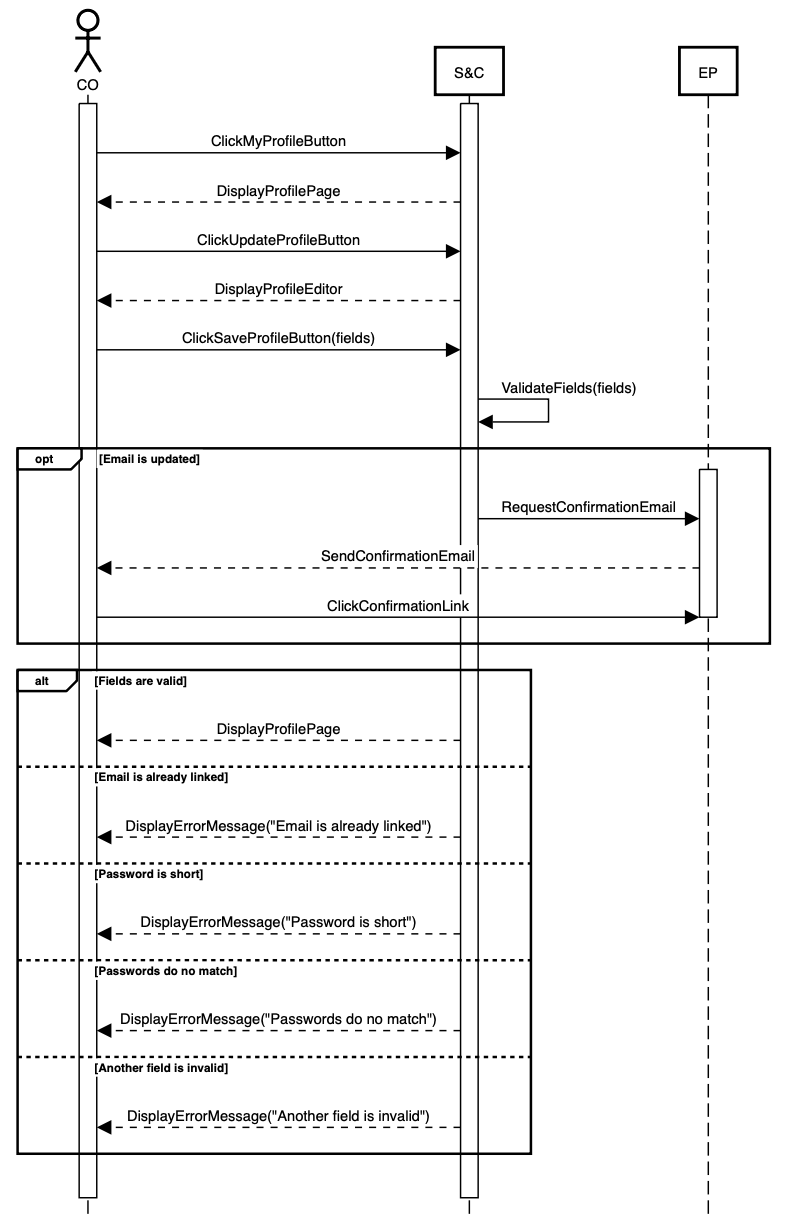
\includegraphics[width=14cm]{images/sequence-diagrams/company-updates-profile.png}
    \caption{UC\theuc\ sequence diagram}
\end{figure}

\stepcounter{uc}

\clearpage
\begin{longtable}{|l|p{10.5cm}|}
    \hline \rowcolor{polimiblue!40}
    \multicolumn{2}{|c|}{\textbf{UC\theuc. Company Posts Position}} \\ \hline
    \textbf{Actors} & CO \\ \hline
    \textbf{Entry Conditions} &  The CO is logged in and S\&C displays the home page. \\ \hline
    \textbf{Event Flow} &
        \begin{minipage}[t]{\linewidth}
            \vspace{10pt}
            \vspace{-\baselineskip}
            \begin{enumerate}[leftmargin=*]
                \item The CO clicks the "Post an Position" button.
                \item S\&C displays the PO posting page.
                \item The CO enters the PO name, domain, project, tasks and terms.
                \item The CO clicks the "Post" button.
                \item S\&C validates the fields.
                \item S\&C displays the home page.
            \end{enumerate}
            \vspace{10pt}
        \end{minipage} \\ \hline
    \textbf{Exit Condition} & The PO is posted and S\&C displays the home page. \\ \hline
    \textbf{Exceptions} &
        \begin{minipage}[t]{\linewidth}
            \vspace{10pt}
            \vspace{-\baselineskip}
            \begin{itemize}[leftmargin=*, label=\tiny\textbullet]
                \item A field is invalid.
            \end{itemize}
            In this case, S\&C displays a descriptive error message.
            \vspace{10pt}
        \end{minipage} \\ \hline
\caption{Use case \theuc}
\end{longtable}

\begin{figure}
    \centering
    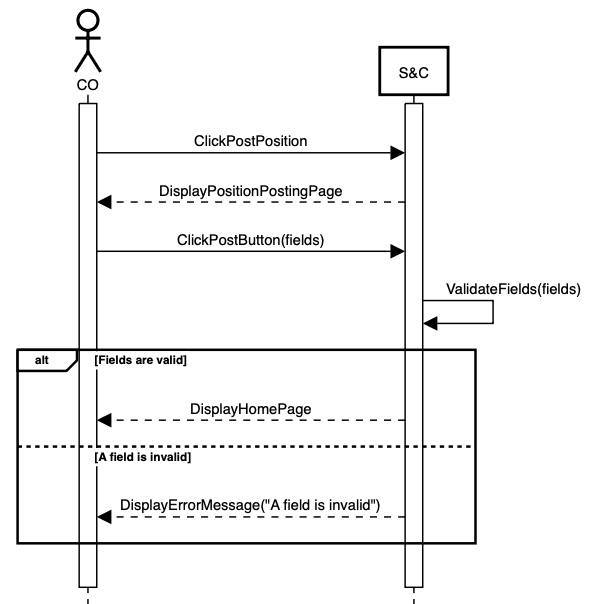
\includegraphics[width=11cm]{images/sequence-diagrams/company-posts-position.png}
    \caption{UC\theuc\ sequence diagram}
\end{figure}

\stepcounter{uc}

\clearpage
\begin{longtable}{|l|p{10.5cm}|}
    \hline \rowcolor{polimiblue!40}
    \multicolumn{2}{|c|}{\textbf{UC\theuc. Company Removes Position}} \\ \hline
    \textbf{Actors} & CO \\ \hline
    \textbf{Entry Conditions} & The CO is logged in, has posted the PO and S\&C displays the home page. \\ \hline
    \textbf{Event Flow} &
        \begin{minipage}[t]{\linewidth}
            \vspace{10pt}
            \vspace{-\baselineskip}
            \begin{enumerate}[leftmargin=*]
                \item The CO clicks the "My Positions" button.
                \item S\&C the POs page.
                \item The CO clicks the PO name.
                \item S\&C displays PO page.
                \item The CO clicks the "Remove Position" button.
                \item S\&C displays POs page.
            \end{enumerate}
            \vspace{10pt}
        \end{minipage} \\ \hline
    \textbf{Exit Condition} & The PO is removed and S\&C displays the POs page. \\ \hline
    \textbf{Exceptions} &
        \begin{minipage}[t]{\linewidth}
            \vspace{10pt}
            \vspace{-\baselineskip}
            None.
            \vspace{10pt}
        \end{minipage} \\ \hline
\caption{Use case \theuc}
\end{longtable}

\begin{figure}[h]
    \centering
    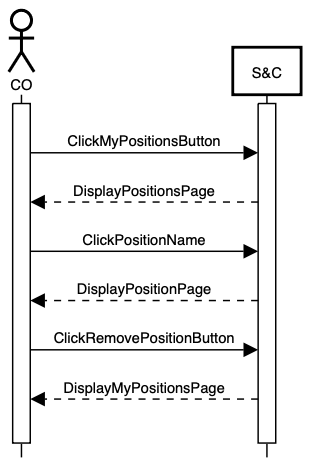
\includegraphics[width=6cm]{images/sequence-diagrams/company-removes-position.png}
    \caption{UC\theuc\ sequence diagram}
\end{figure}

\stepcounter{uc}

\clearpage
\begin{longtable}{|l|p{10.5cm}|}
    \hline \rowcolor{polimiblue!40}
    \multicolumn{2}{|c|}{\textbf{UC\theuc. Company Views Company}} \\ \hline
    \textbf{Actors} & CO \\ \hline
    \textbf{Entry Condition} & The CO is logged in and S\&C displays the US name. \\ \hline
    \textbf{Event Flow} &
        \begin{minipage}[t]{\linewidth}
            \vspace{10pt}
            \vspace{-\baselineskip}
            \begin{enumerate}[leftmargin=*]
                \item The CO clicks the US name.
                \item S\&C displays the US page.
            \end{enumerate}
            \vspace{10pt}
        \end{minipage} \\ \hline
    \textbf{Exit Condition} & S\&C displays the US page. \\ \hline
    \textbf{Exceptions} &
        \begin{minipage}[t]{\linewidth}
            \vspace{10pt}
            \vspace{-\baselineskip}
            \begin{itemize}[leftmargin=*, label=\tiny\textbullet]
                \item The US has been deleted.
            \end{itemize}
            In this case, S\&C displays a descriptive error message.
            \vspace{10pt}
        \end{minipage} \\ \hline
\caption{Use case \theuc}
\end{longtable}

\begin{figure}[h]
    \centering
    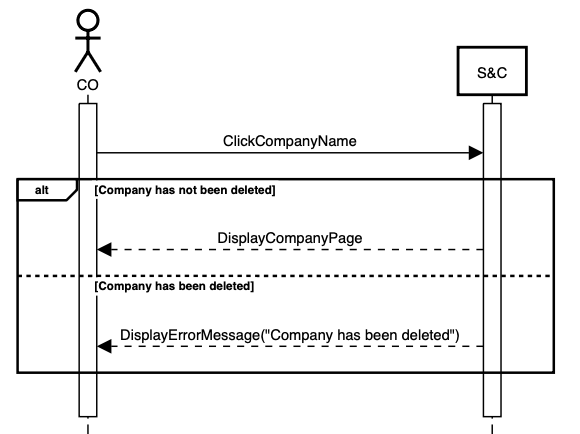
\includegraphics[width=11cm]{images/sequence-diagrams/company-views-student.png}
    \caption{UC\theuc\ sequence diagram}
\end{figure}

\stepcounter{uc}

\clearpage
\begin{longtable}{|l|p{10.5cm}|}
    \hline \rowcolor{polimiblue!40}
    \multicolumn{2}{|c|}{\textbf{UC\theuc. Company Accepts Recommendation}} \\ \hline
    \textbf{Actors} & CO, US, EP \\ \hline
    \textbf{Entry Condition} & The CO is logged in and has ticked the "Keep Me Updated" field. \\ \hline
    \textbf{Event Flow} &
        \begin{minipage}[t]{\linewidth}
            \vspace{10pt}
            \vspace{-\baselineskip}
            \begin{enumerate}[leftmargin=*]
                \item S\&C sends a notification email to the CO via the EP.
                \item The CO clicks the "View Student" link on the email.
                \item S\&C displays the US page.
                \item The CO clicks the "Accept" button.
                \item S\&C displays the PO page.
                \item S\&C checks if a match is identified.
                \item S\&C sends a notification email to the CO via the EP.
                \item S\&C sends a notification email to the US via the EP.
            \end{enumerate}
            \vspace{10pt}
        \end{minipage} \\ \hline
    \textbf{Exit Condition} & The recommendation is accepted and S\&C displays the PO page. \\ \hline
    \textbf{Exceptions} &
        \begin{minipage}[t]{\linewidth}
            \vspace{10pt}
            \vspace{-\baselineskip}
            \begin{itemize}[leftmargin=*, label=\tiny\textbullet]
                \item The recommendation has already been resolved.
                \item The US has been deleted.
            \end{itemize}
            In all cases, S\&C displays the home page and a descriptive error message.
            \vspace{10pt}
        \end{minipage} \\ \hline
\caption{Use case \theuc}
\end{longtable}

\begin{figure}
    \centering
    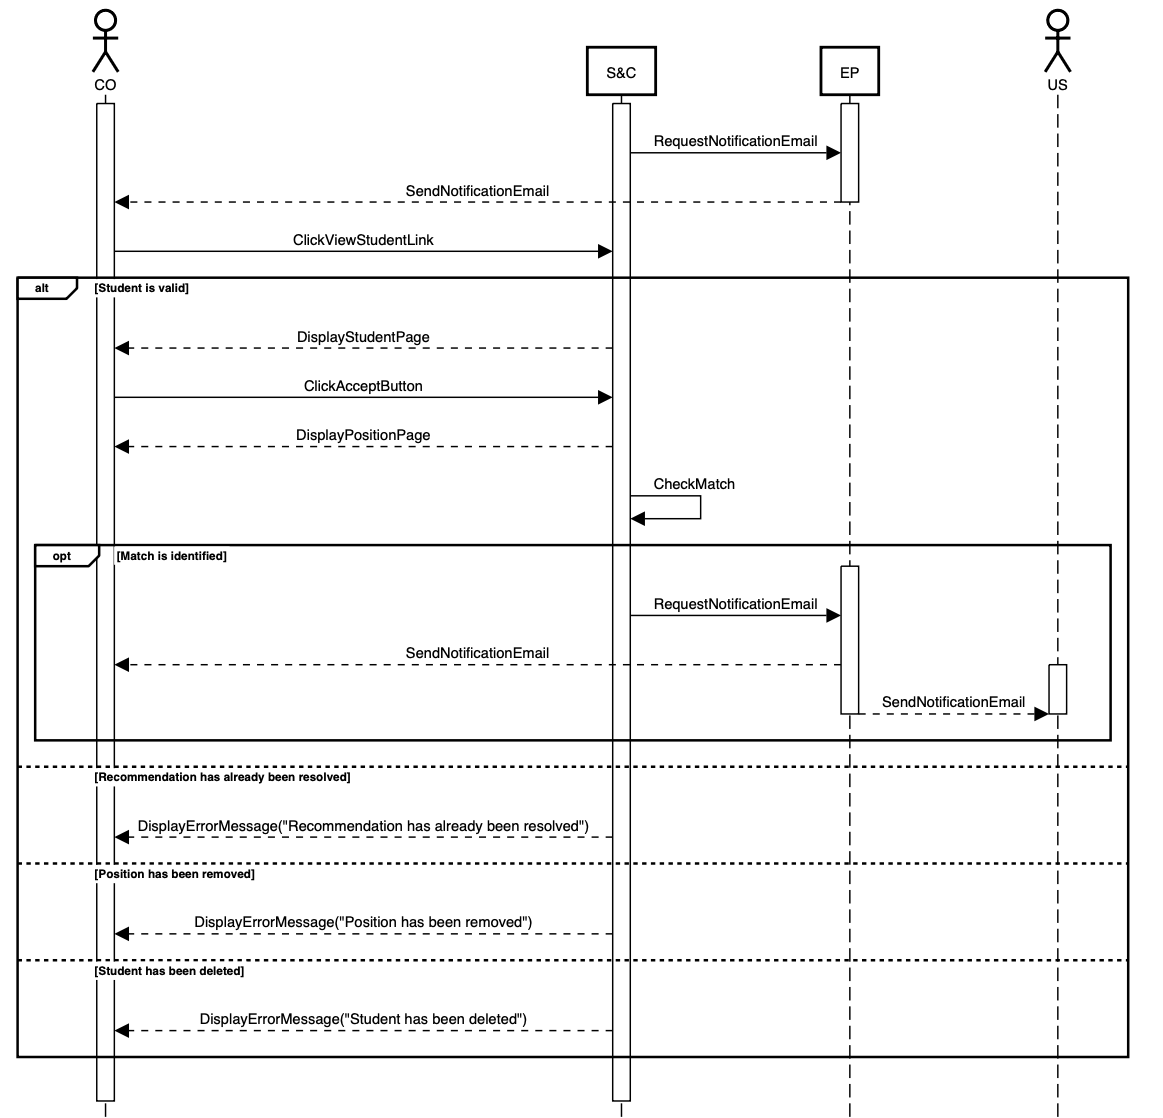
\includegraphics[width=16cm]{images/sequence-diagrams/company-accepts-recommendation.png}
    \caption{UC\theuc\ sequence diagram}
\end{figure}

\stepcounter{uc}

\clearpage
\begin{longtable}{|l|p{10.5cm}|}
    \hline \rowcolor{polimiblue!40}
    \multicolumn{2}{|c|}{\textbf{UC\theuc. Company Fills Out Feedback Form}} \\ \hline
    \textbf{Actors} & US \\ \hline
    \textbf{Entry Condition} & The CO is logged in and S\&C displays the home page. \\ \hline
    \textbf{Event Flow} &
        \begin{minipage}[t]{\linewidth}
            \vspace{10pt}
            \vspace{-\baselineskip}
            \begin{enumerate}[leftmargin=*]
                \item The CO clicks the "Give Feedback" button.
                \item S\&C displays the feedback form.
                \item The CO enters the fields.
                \item The CO clicks the "Submit" button.
                \item S\&C validates the fields.
                \item S\&C displays the home page.
            \end{enumerate}
            \vspace{10pt}
        \end{minipage} \\ \hline
    \textbf{Exit Condition} & The feedback form is submitted and S\&C displays the home page. \\ \hline
    \textbf{Exceptions} &
        \begin{minipage}[t]{\linewidth}
            \vspace{10pt}
            \vspace{-\baselineskip}
            \begin{itemize}[leftmargin=*, label=\tiny\textbullet]
                \item A field is invalid.
            \end{itemize}
            In this case, S\&C displays a descriptive error message.
            \vspace{10pt}
        \end{minipage} \\ \hline
\caption{Use case \theuc}
\end{longtable}

\begin{figure}[h]
    \centering
    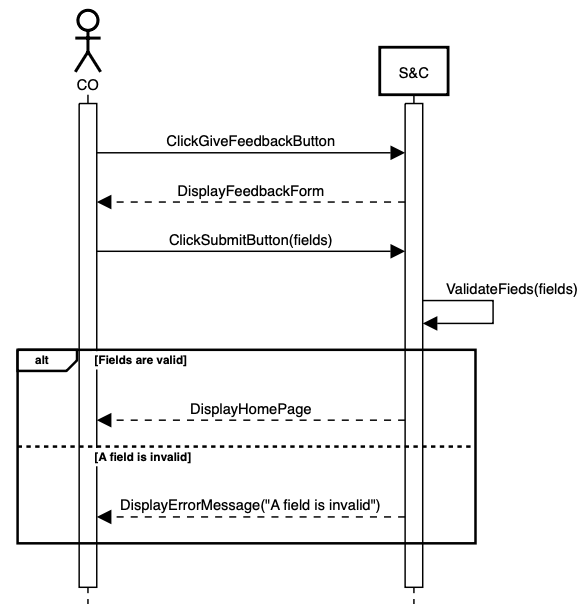
\includegraphics[width=11cm]{images/sequence-diagrams/company-fills-out-feedback-form.png}
    \caption{UC\theuc\ sequence diagram}
\end{figure}

\stepcounter{uc}

\clearpage
\begin{longtable}{|l|p{10.5cm}|}
    \hline \rowcolor{polimiblue!40}
    \multicolumn{2}{|c|}{\textbf{UC\theuc. Company Adds Questionnaire}} \\ \hline
    \textbf{Actors} & CO, US, EP \\ \hline
    \textbf{Entry Conditions} & The CO is logged in, has posted the PO and S\&C displays the home page. \\ \hline
    \textbf{Event Flow} &
        \begin{minipage}[t]{\linewidth}
            \vspace{10pt}
            \vspace{-\baselineskip}
            \begin{enumerate}[leftmargin=*]
                \item The CO clicks on the "My Positions" button.
                \item S\&C displays the POs page.
                \item The CO clicks on the PO name.
                \item S\&C displays the PO page.
                \item The CO clicks on the "Add Questionnaire" button.
                \item S\&C displays the questionnaire editor.
                \item The CO edits the questionnaire.
                \item The CO clicks the "Add" button.
                \item S\&C displays the PO page.
                \item S\&C sends a notification email to USs via the EP.
            \end{enumerate}
            \vspace{10pt}
        \end{minipage} \\ \hline
    \textbf{Exit Condition} & The questionnaire is added, USs are notified and S\&C displays the PO page. \\ \hline
    \textbf{Exceptions} &
        \begin{minipage}[t]{\linewidth}
            \vspace{10pt}
            \vspace{-\baselineskip}
            \begin{itemize}[leftmargin=*, label=\tiny\textbullet]
                \item A field is invalid.
            \end{itemize}
            In this case, S\&C displays a descriptive error message.
            \vspace{10pt}
        \end{minipage} \\ \hline
\caption{Use case \theuc}
\end{longtable}

\begin{figure}
    \centering
    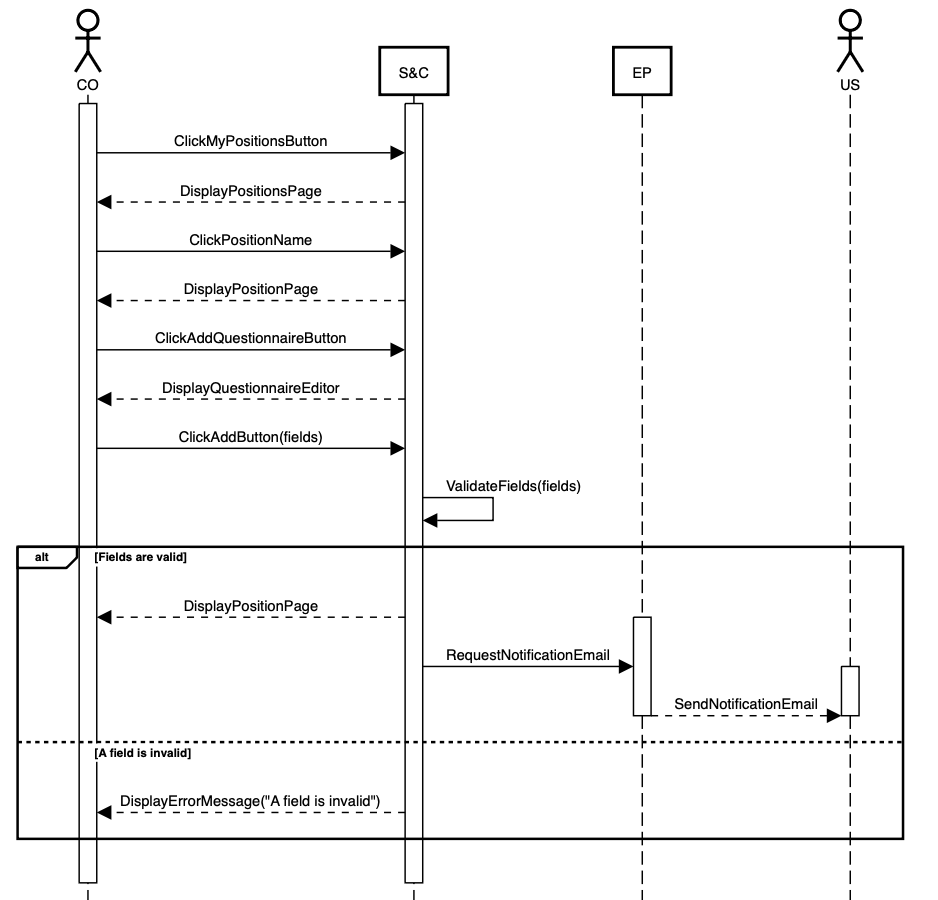
\includegraphics[width=16cm]{images/sequence-diagrams/company-adds-questionnaire.png}
    \caption{UC\theuc\ sequence diagram}
\end{figure}

\stepcounter{uc}

\clearpage
\begin{longtable}{|l|p{10.5cm}|}
    \hline \rowcolor{polimiblue!40}
    \multicolumn{2}{|c|}{\textbf{UC\theuc. Company Schedules Interview}} \\ \hline
    \textbf{Actors} & CO, US, EP \\ \hline
    \textbf{Entry Conditions} & The CO is logged in, has posted the PO and S\&C displays the home page. \\ \hline
    \textbf{Event Flow} &
        \begin{minipage}[t]{\linewidth}
            \vspace{10pt}
            \vspace{-\baselineskip}
            \begin{enumerate}[leftmargin=*]
                \item The CO clicks on the "My Positions" button.
                \item S\&C displays the POs page.
                \item The CO clicks on the PO name.
                \item S\&C displays the PO page.
                \item The CO clicks on the US name.
                \item S\&C displays the US page.
                \item The CO clicks on the "Schedule an Interview" button.
                \item S\&C displays the interview form.
                \item The CO enters the date and the mode.
                \item The CO clicks the "Schedule" button.
                \item S\&C validates the fields.
                \item S\&C displays the US page.
                \item S\&C sends a notification email to the US via the EP.
            \end{enumerate}
            \vspace{10pt}
        \end{minipage} \\ \hline
    \textbf{Exit Condition} & The interview is scheduled, the US is notified and S\&C displays the US page. \\ \hline
    \textbf{Exceptions} &
        \begin{minipage}[t]{\linewidth}
            \vspace{10pt}
            \vspace{-\baselineskip}
            \begin{itemize}[leftmargin=*, label=\tiny\textbullet]
                \item The date is in the past.
                \item The mode is invalid.
            \end{itemize}
            In this case, S\&C displays a descriptive error message.
            \vspace{10pt}
        \end{minipage} \\ \hline
\caption{Use case \theuc}
\end{longtable}

\begin{figure}
    \centering
    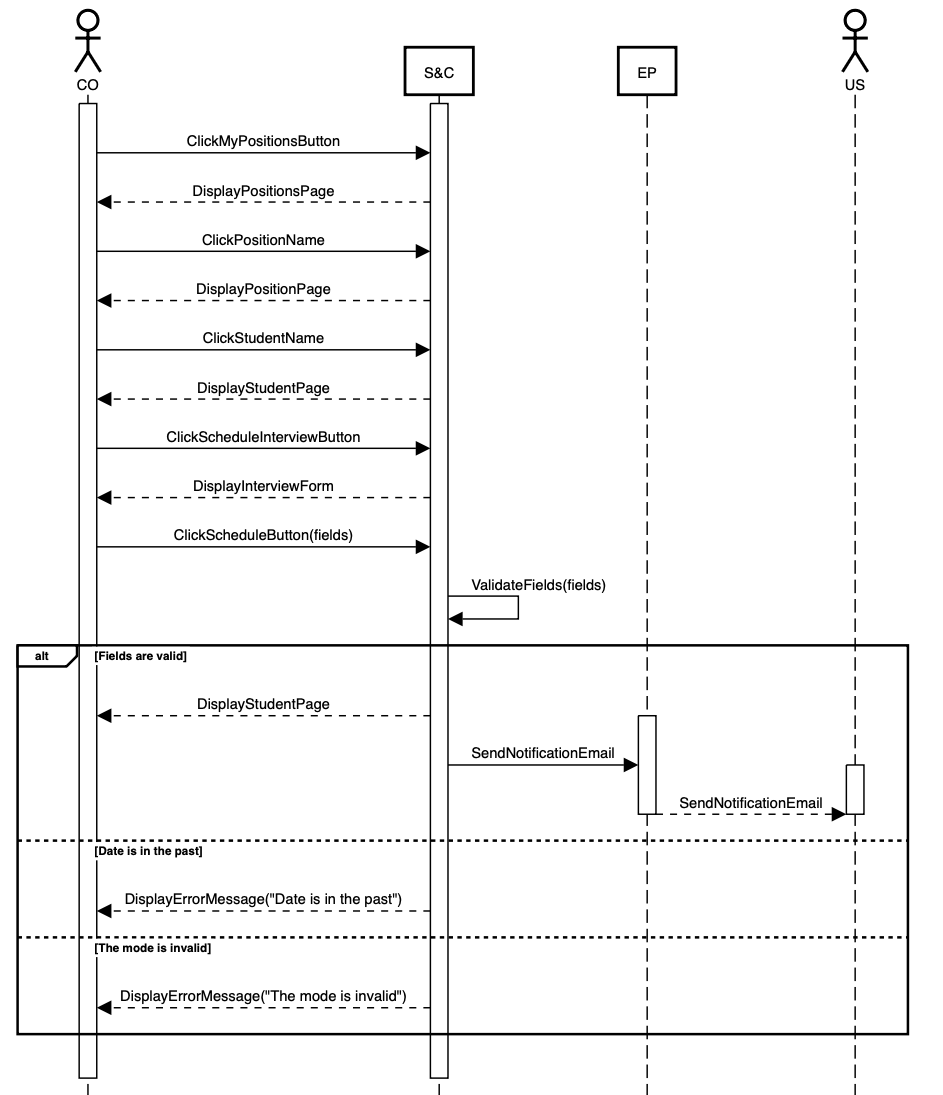
\includegraphics[width=16cm]{images/sequence-diagrams/company-schedules-interview.png}
    \caption{UC\theuc\ sequence diagram}
\end{figure}

\stepcounter{uc}

\clearpage
\begin{longtable}{|l|p{10.5cm}|}
    \hline \rowcolor{polimiblue!40}
    \multicolumn{2}{|c|}{\textbf{UC\theuc. Company Comments Internship}} \\ \hline
    \textbf{Actors} & US, CO, UN, EP \\ \hline
    \textbf{Entry Conditions} & The CO is logged in, hosting an IN and S\&C displays the home page. \\ \hline
    \textbf{Event Flow} &
        \begin{minipage}[t]{\linewidth}
            \vspace{10pt}
            \vspace{-\baselineskip}
            \begin{enumerate}[leftmargin=*]
                \item The CO clicks the "My Internships" button.
                \item S\&C displays the internships page.
                \item The CO clicks the IN name.
                \item S\&C displays the IN page.
                \item The CO clicks the "Write a Comment" button.
                \item S\&C displays the comment form.
                \item The CO enters the fields.
                \item The CO clicks the "Send" button.
                \item S\&C validates the fields.
                \item S\&C displays the IN page.
                \item S\&C sends a notification email to the US via the EP.
                \item S\&C sends a notification email to the UN via the EP.
            \end{enumerate}
            \vspace{10pt}
        \end{minipage} \\ \hline
    \textbf{Exit Condition} & The comment is sent, the US and the UN are notified and S\&C displays the IN page. \\ \hline
    \textbf{Exceptions} &
        \begin{minipage}[t]{\linewidth}
            \vspace{10pt}
            \vspace{-\baselineskip}
            \begin{itemize}[leftmargin=*, label=\tiny\textbullet]
                \item A field is invalid.
            \end{itemize}
            In this case, S\&C displays a descriptive error message.
            \vspace{10pt}
        \end{minipage} \\ \hline
\caption{Use case \theuc}
\end{longtable}

\begin{figure}
    \centering 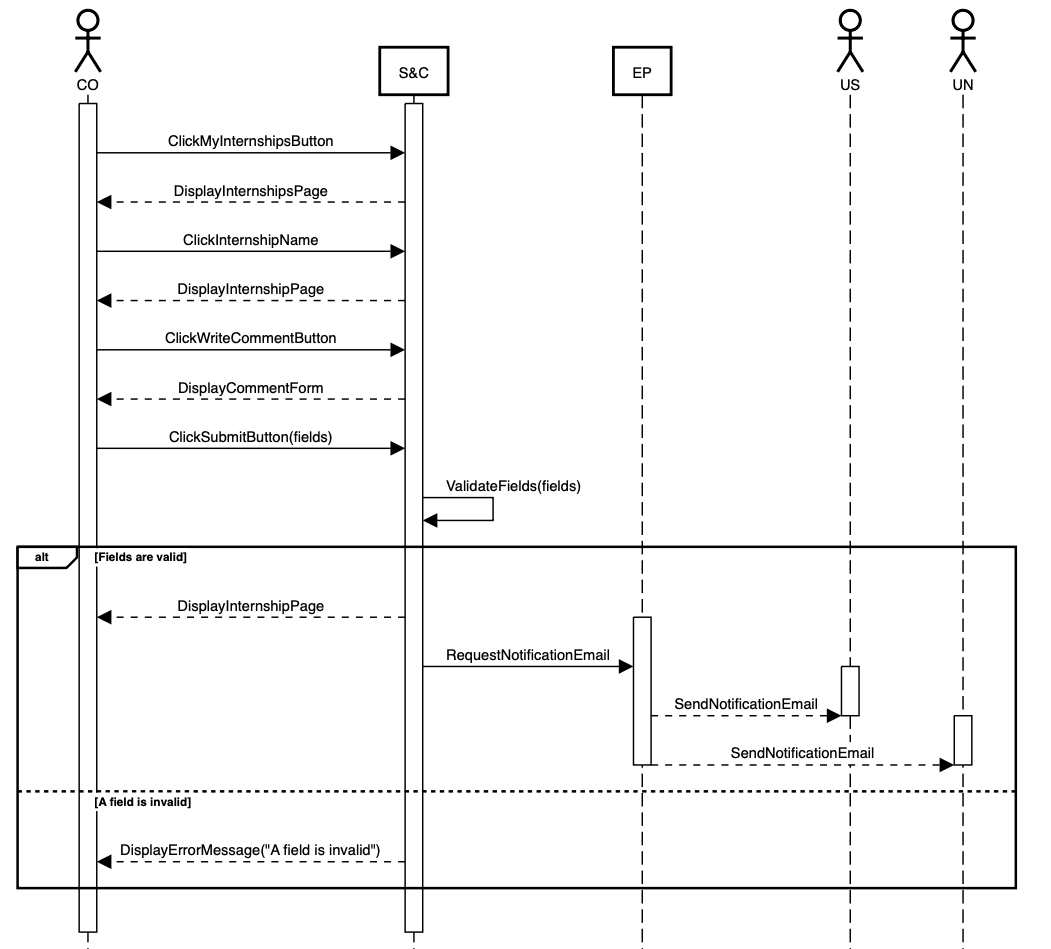
\includegraphics[width=16cm]{images/sequence-diagrams/company-comments-internship.png}
    \caption{UC\theuc\ sequence diagram}
\end{figure}

\stepcounter{uc}

\clearpage
\subsubsection{University Use Cases}
The following use case diagram depicts the main activities a university can carry out.

\begin{figure}[h]
   \centering    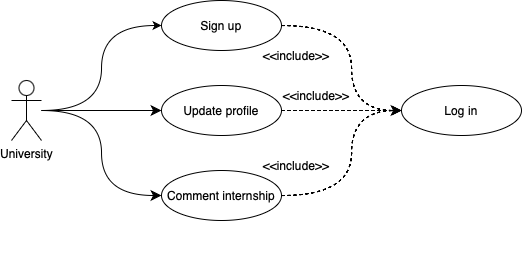
\includegraphics[width=10cm]{images/use-case-diagrams/university.png}
    \caption{University use cases diagram}
\end{figure}

\clearpage
\begin{longtable}{|l|p{10.5cm}|}
    \hline \rowcolor{polimiblue!40}
    \multicolumn{2}{|c|}{\textbf{UC\theuc. University Signs Up}} \\ \hline
    \textbf{Actors} & UN, EP \\ \hline
    \textbf{Entry Conditions} & The UN is not signed up on S\&C. \\ \hline
    \textbf{Event Flow} &
        \begin{minipage}[t]{\linewidth}
            \vspace{10pt}
            \vspace{-\baselineskip}
            \begin{enumerate}[leftmargin=*]
                \item The UN navigates to the landing page.
                \item S\&C displays the landing page.
                \item The UN clicks the "Sign Up as a University" button.
                \item S\&C displays the signup page.
                \item The UN enters his name, institutional email address, password and confirms the password.
                \item The UN can tick the "Keep Me Updated" field.
                \item The UN clicks the "Sign Up" button.
                \item S\&C validates the fields.
                \item S\&C sends a confirmation email to the UN via the EP.
                \item The UN clicks the confirmation link in the email.
                \item S\&C displays the login page.
            \end{enumerate}
            \vspace{10pt}
        \end{minipage} \\ \hline
    \textbf{Exit Condition} & The UN is signed up and S\&C displays the login page. \\ \hline
    \textbf{Exceptions} &
        \begin{minipage}[t]{\linewidth}
            \vspace{10pt}
            \vspace{-\baselineskip}
            \begin{itemize}[leftmargin=*, label=\tiny\textbullet]
                \item The email is not a valid institutional email address.
                \item The email is already linked to another profile.
                \item The password is shorter than 8 characters.
                \item The passwords do not match.
                \item Another field is invalid.
            \end{itemize}
            In all cases, S\&C displays a descriptive error message.
            \vspace{10pt}
        \end{minipage} \\ \hline
\caption{Use case \theuc}
\end{longtable}

\begin{figure}
    \centering
    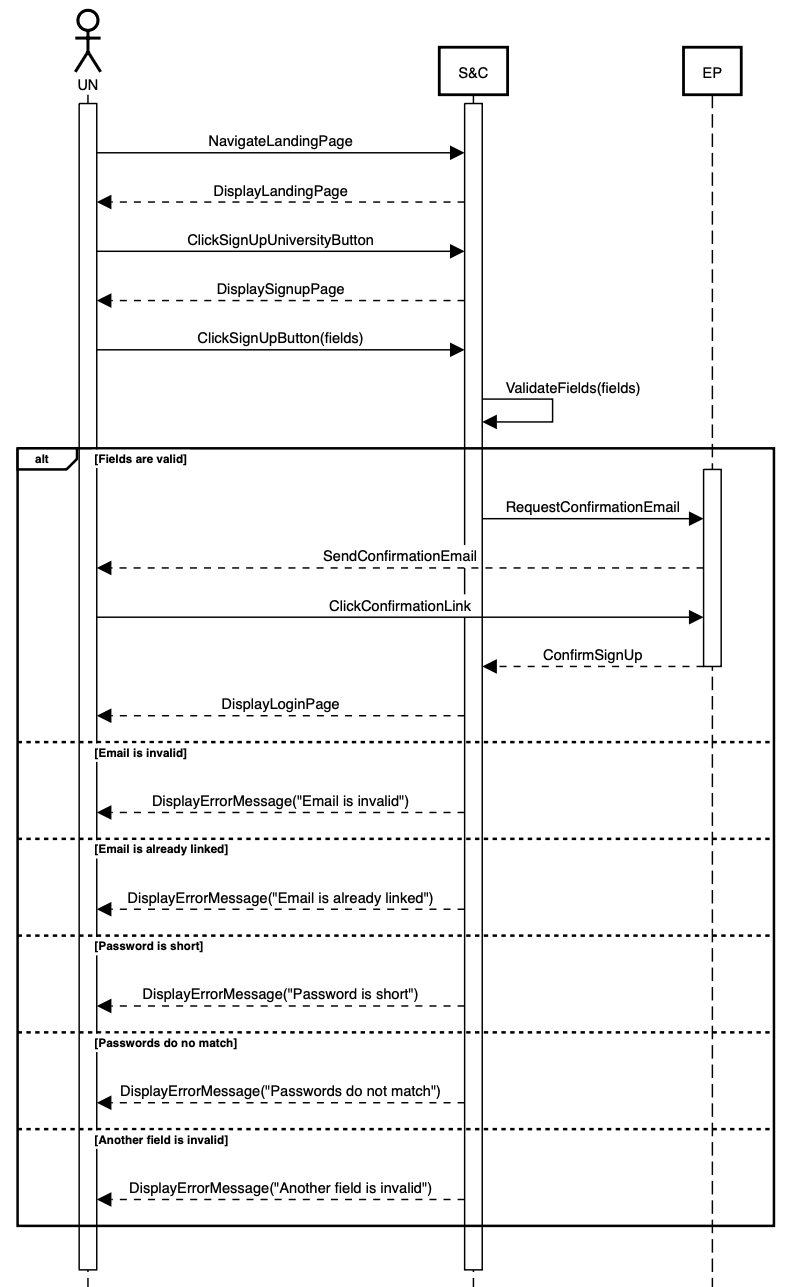
\includegraphics[width=13cm]{images/sequence-diagrams/university-signs-up.png}
    \caption{UC\theuc\ sequence diagram}
\end{figure}

\stepcounter{uc}

\clearpage
\begin{longtable}{|l|p{10.5cm}|}
    \hline \rowcolor{polimiblue!40}
    \multicolumn{2}{|c|}{\textbf{UC\theuc. University Updates Profile}} \\ \hline
    \textbf{Actors} & UN \\ \hline
    \textbf{Entry Condition} & The UN is logged in and S\&C displays the home page. \\ \hline
    \textbf{Event Flow} &
        \begin{minipage}[t]{\linewidth}
            \vspace{10pt}
            \vspace{-\baselineskip}
            \begin{enumerate}[leftmargin=*]
                \item The UN clicks the "My Profile" button.
                \item S\&C displays the profile page.
                \item The UN clicks the "Update Profile" button.
                \item S\&C displays the profile editor.
                \item The UN updates the desired fields.
                \item The UN clicks the "Save Profile" button.
                \item S\&C validates the fields.
                \item S\&C displays the profile page.
            \end{enumerate}
            \vspace{10pt}
        \end{minipage} \\ \hline
    \textbf{Exit Condition} & The profile is updated and S\&C displays the profile page. \\ \hline
    \textbf{Exceptions} &
        \begin{minipage}[t]{\linewidth}
            \vspace{10pt}
            \vspace{-\baselineskip}
            \begin{itemize}[leftmargin=*, label=\tiny\textbullet]
                \item The email is not a valid institutional email address.
                \item The email is already linked to another profile.
                \item The password is shorter than 8 characters.
                \item The passwords do not match.
                \item Another field is invalid.
            \end{itemize}
            In all cases, S\&C displays a descriptive error message.
            \vspace{10pt}
        \end{minipage} \\ \hline
\caption{Use case \theuc}
\end{longtable}

\begin{figure}
    \centering
    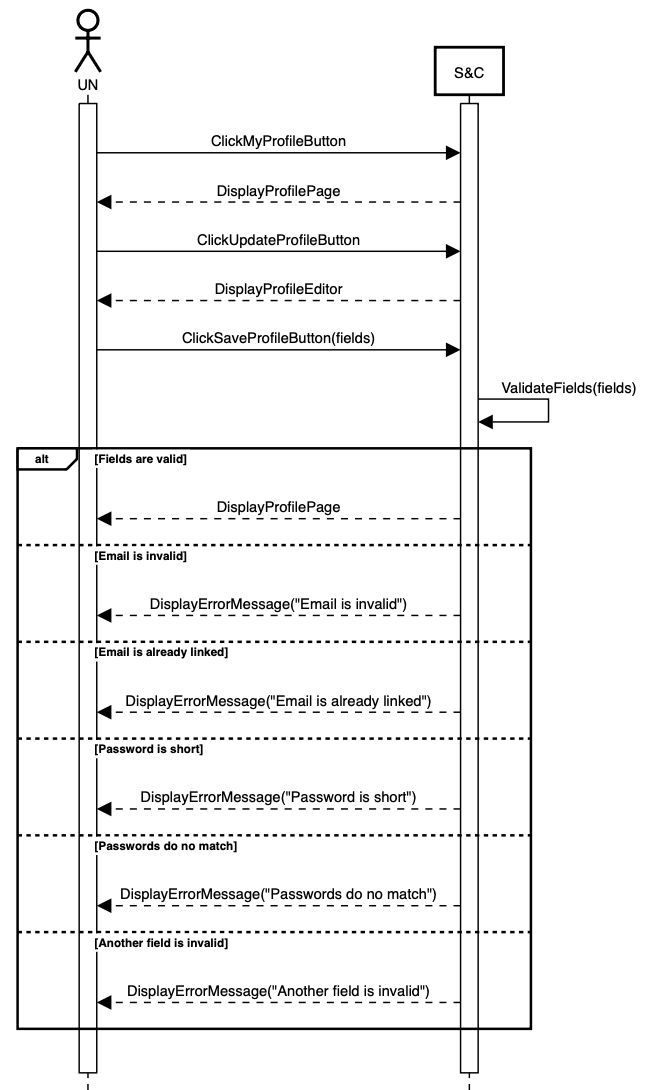
\includegraphics[width=12cm]{images/sequence-diagrams/university-updates-profile.png}
    \caption{UC\theuc\ sequence diagram}
\end{figure}

\stepcounter{uc}

\clearpage
\begin{longtable}{|l|p{10.5cm}|}
    \hline \rowcolor{polimiblue!40}
    \multicolumn{2}{|c|}{\textbf{UC\theuc. University Comments Internship}} \\ \hline
    \textbf{Actors} & UN, US, CO, EP \\ \hline
    \textbf{Entry Conditions} & The UN is logged in and S\&C displays the home page. \\ \hline
    \textbf{Event Flow} &
        \begin{minipage}[t]{\linewidth}
            \vspace{10pt}
            \vspace{-\baselineskip}
            \begin{enumerate}[leftmargin=*]
                \item The UN clicks the US name.
                \item S\&C displays the US page.
                \item The UN clicks the IN name.
                \item S\&C displays the IN page.
                \item The UN clicks the "Write a Comment" button.
                \item S\&C displays the the comment form.
                \item The UN enters the fields.
                \item The UN clicks the "Send" button.
                \item S\&C checks the fields.
                \item S\&C displays the IN page.
                \item S\&C sends a notification email to the US via the EP.
                \item S\&C sends a notification email to the CO via the EP.
            \end{enumerate}
            \vspace{10pt}
        \end{minipage} \\ \hline
    \textbf{Exit Condition} & The comment is sent, the US and the CO are notified and S\&C displays the IN page. \\ \hline
    \textbf{Exceptions} &
        \begin{minipage}[t]{\linewidth}
            \vspace{10pt}
            \vspace{-\baselineskip}
            \begin{itemize}[leftmargin=*, label=\tiny\textbullet]
                \item A field is invalid.
            \end{itemize}
            In this case, S\&C displays a descriptive error message.
            \vspace{10pt}
        \end{minipage} \\ \hline
\caption{Use case \theuc}
\end{longtable}

\begin{figure}[h]
    \centering
    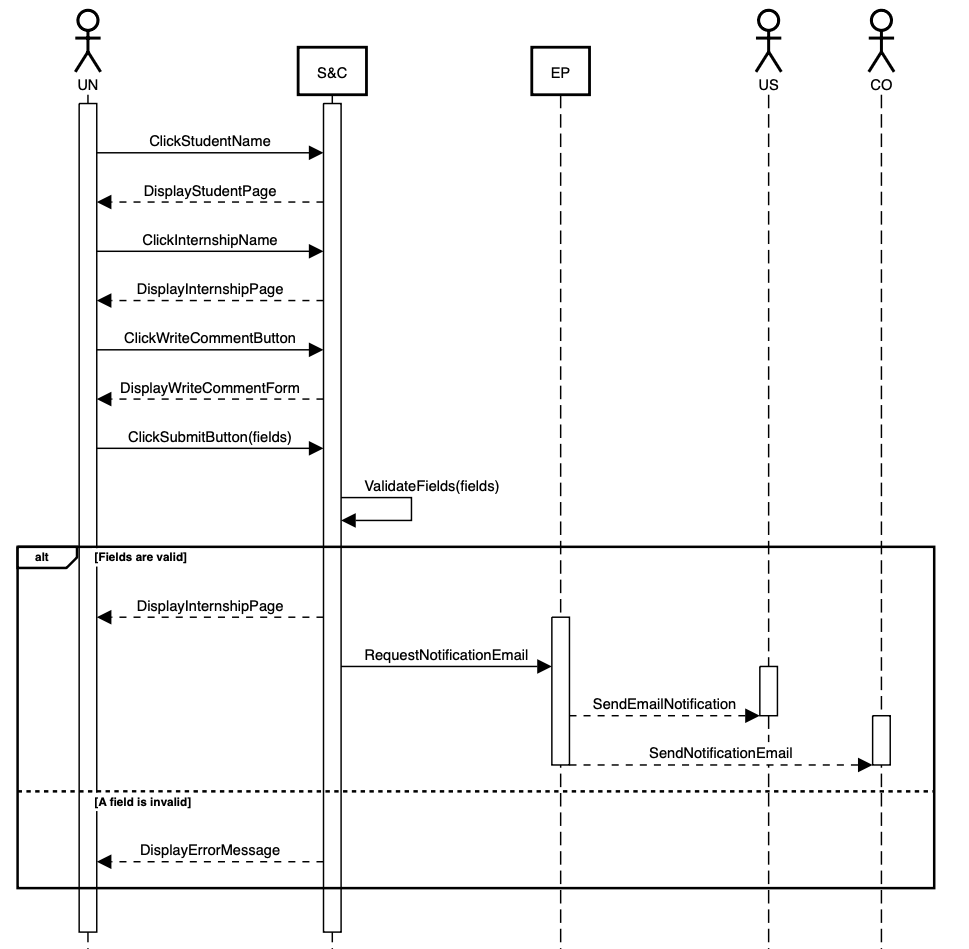
\includegraphics[width=16cm]{images/sequence-diagrams/university-comments-internship.png}
    \caption{UC\theuc\ sequence diagram}
\end{figure}

\clearpage
